\section{Configuration Parameters}
Configuration parameters for seismic hazard calculations can be broadly divided into five main groups:
\begin{itemize}
\item Source Model parameters
\item GMPE parameters
\item Site parameters
\item Logic Tree parameters
\item Calculator specific parameters
\end{itemize}

\subsection{Source Model parameters}
Source Model parameters define how seismic sources are modeled by the engine in order to create the earthquake rupture forecast (ERF).\\
\subsubsection{Area source parameters}
Each source typology has its own set of parameters. For area sources, the following parameters must be set:
\begin{itemize}
\item \Verb+INCLUDE_AREA_SOURCES+: if \Verb+true+ all area sources in the source model are included in the ERF calculation. They are exclude if \Verb+false+.
\item \Verb+TREAT_AREA_SOURCE_AS+: specifies how ruptures in area sources must be modeled. Allowed values are:
\begin{itemize}
\item \Verb+Point Sources+
\item \Verb+Line Sources (random or given strike)+
\item \Verb+Cross Hair Line Sources+
\item \Verb+16 Spoked Line Sources+
\end{itemize}
\item \Verb+AREA_SOURCE_DISCRETIZATION+: defines area source region discretization step (in decimal degrees). Minimum value is 0.01. Typical value is 0.1.
\item \Verb+AREA_SOURCE_MAGNITUDE_SCALING_RELATIONSHIP+: specifies the magnitude scaling relationship used for modeling finite ruptures. It can be only a magnitude-length relationship (list of available scaling relationships are given in Appendix B).
\end{itemize}
Figure \ref{areaSrcGridSpacing} shows the effect of the area source discretization parameter. Given the area boundary (white polygon), ruptures' hypocenters are placed inside the area on a regular grid of nodes (red dots), whose spacing is determined by the area discretization value. Smaller is the grid spacing better the earthquake ruptures cover the area polygon, however higher is the number of ruptures to be considered in the ERF (hence higher is the computation time).\\
\begin{figure}[!htbp]
\begin{center}
\subfigure[]{
\includegraphics[width=6cm]{./oqum_Figures/areaSrcGrid01.eps}}
\subfigure[]{
\includegraphics[width=6cm]{./oqum_Figures/areaSrcGrid005.eps}}\\
\caption{Area source discretization. Decreasing discretization step [from (a) to (b)] improves rupture distribution on the area polygon.}
\label{areaSrcGridSpacing}
\end{center}
\end{figure}
Two main options are available for modeling earthquake ruptures inside area sources: point or line. Figure \ref{areaSrcPointVersusLine} depicts the two approaches. If the point rupture option is chosen, earthquake ruptures (independently of their magnitude values) are modeled as points (red dots) located at a depth equal to the hypocentral depth (a). If the line rupture option is chosen, ruptures' hypocenters are modeled as points (red dots) (again at a depth equal to the hypocentral depth). However, for ruptures with magnitudes in the range specified by the rupture depth distribution,  the rupture's top edge is modeled as a line placed at a depth associated to the rupture's magnitude (green and yellow lines represent ruptures' top edges for two magnitude bins in the rupture depth distribution) (b). The finite rupture option allows to model the rupture's hypocenter and top edge, and therefore to honor those GMPEs that make use of both these two pieces of information [for instance focal depth and distance to the rupture (closest distance or JB distance)]. The distance to the rupture is correctly computed for vertical ruptures (dip = 90\degree), however for dipping ruptures (dip $< 90$\degree) the distance calculation is based only on the rupture top edge and ignore the rupture extension along dip.\\
\begin{figure}[!htbp]
\begin{center}
\subfigure[]{
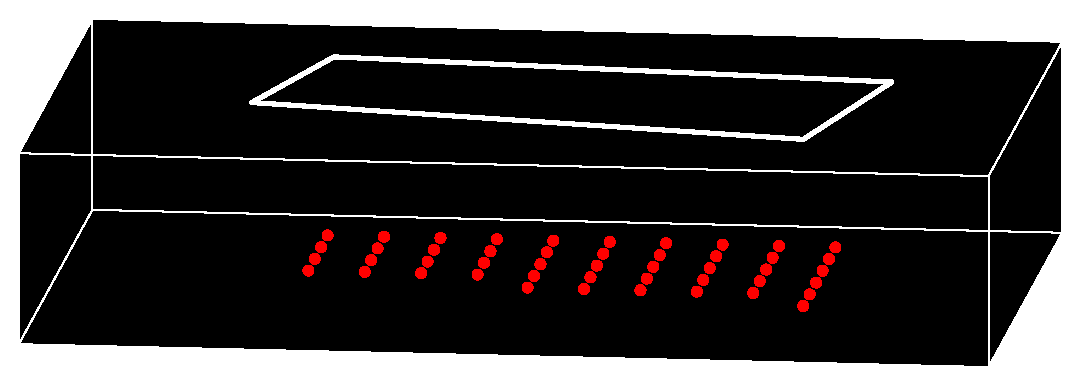
\includegraphics[width=12cm]{./oqum_Figures/areaSrcPointRupture.eps}}
\subfigure[]{
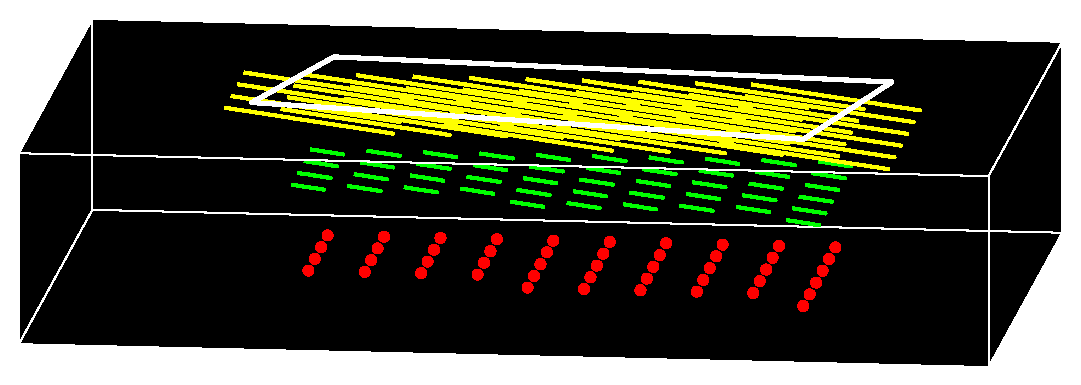
\includegraphics[width=12cm]{./oqum_Figures/areaSrcFiniteRuptureGivenStrike.eps}}
\caption{Point (a) and finite ruptures (b) in area source. }
\label{areaSrcPointVersusLine}
\end{center}
\end{figure}
If the line rupture option is chosen, multiple strategies are available to take into account the rupture orientation. If a strike value is provided, ruptures can be aligned according to it, if it is not a random strike is generated [Figure \ref{areaSrcLineRuptures} (a) and (b)]. Possible alternatives are also distributing ruptures along two perpendicular directions [NS-EW, Figure \ref{areaSrcLineRuptures} (c)], and spin the ruptures over 360\degree [every 22.5 \degree, Figure \ref{areaSrcLineRuptures} (d)]. 
\begin{figure}[!htbp]
\begin{center}
\subfigure[]{
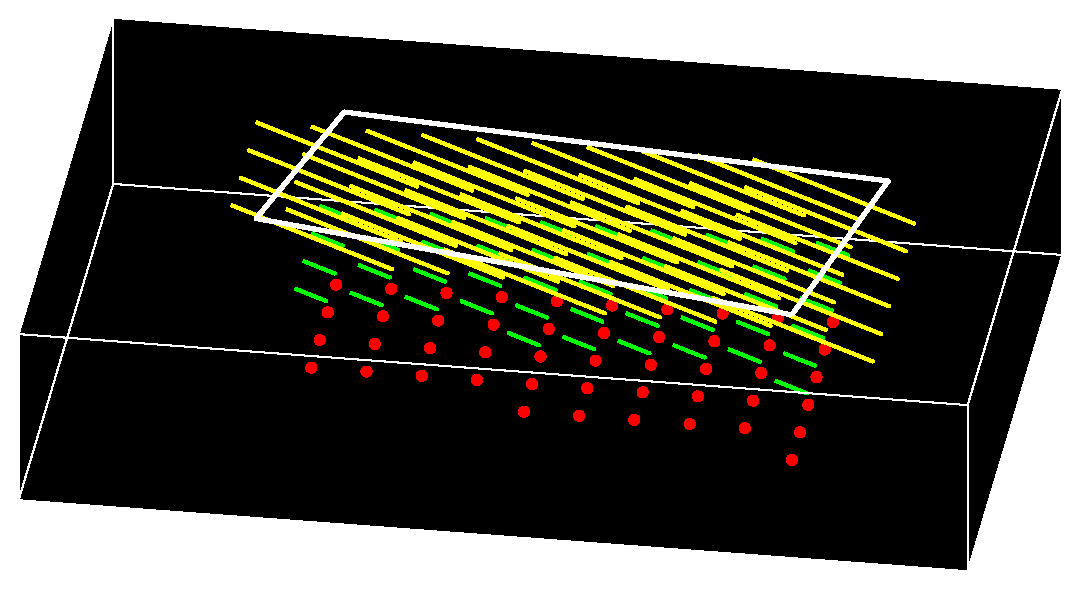
\includegraphics[width=8cm]{./oqum_Figures/areaSrcFiniteRuptureGivenStrike2.eps}}
\subfigure[]{
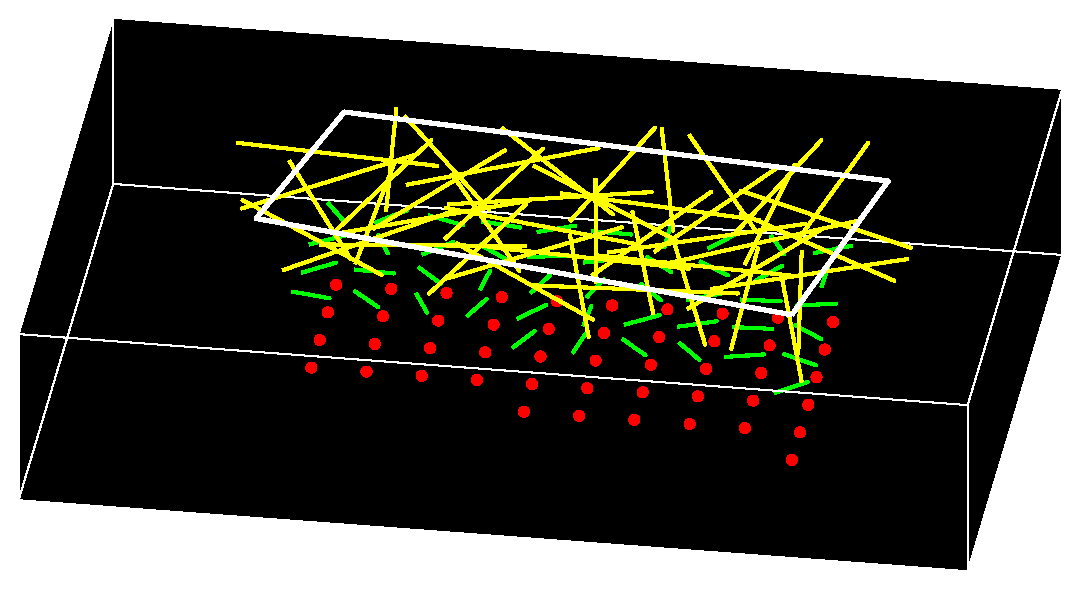
\includegraphics[width=8cm]{./oqum_Figures/areaSrcFiniteRuptureRandom.eps}}
\subfigure[]{
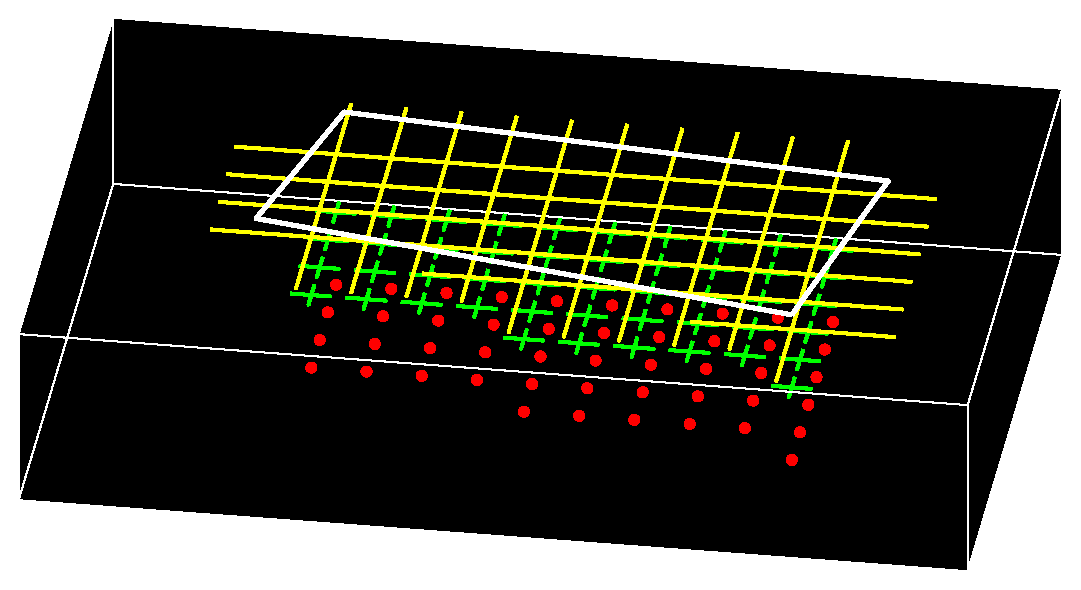
\includegraphics[width=8cm]{./oqum_Figures/areaSrcFiniteRuptureCross.eps}}
\subfigure[]{
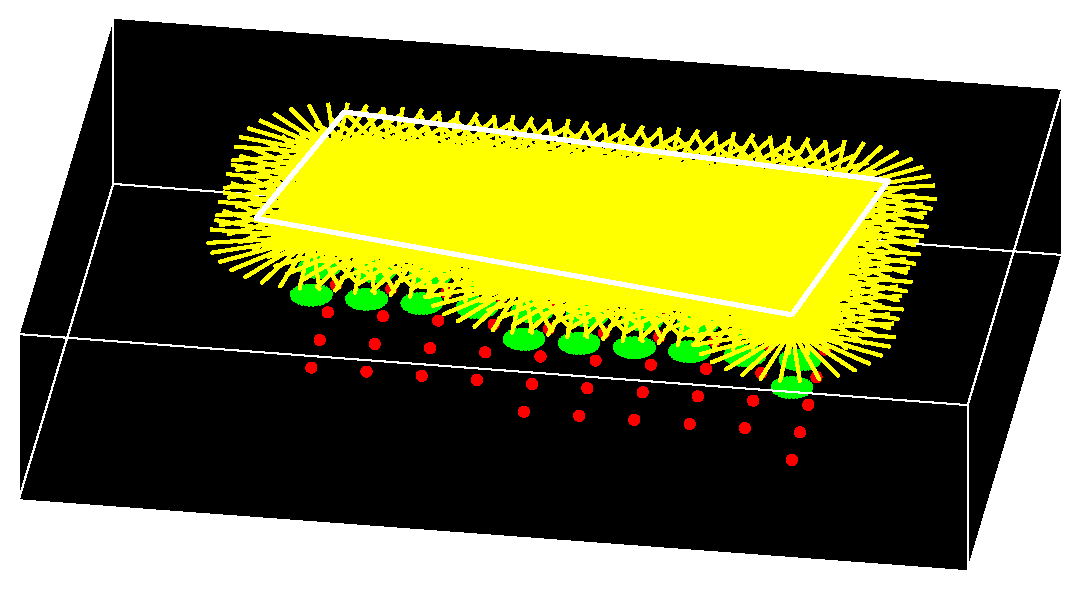
\includegraphics[width=8cm]{./oqum_Figures/areaSrcFiniteRuptureSpoked.eps}}
\caption{Different options for modeling rupture orientation in area source. Along given strike (a), random strike (b), along two perpendicular directions (c), along multiple strikes in the range 0 to 360 \degree (d).}
\label{areaSrcLineRuptures}
\end{center}
\end{figure}

\subsubsection{Point source parameters}
Point sources require similar parameters as area sources:
\begin{itemize}
\item \Verb+INCLUDE_GRID_SOURCES+: if \Verb+true+ all point sources in the source model are included in the ERF calculation. They are exclude if \Verb+false+.
\item \Verb+TREAT_GRID_SOURCE_AS+: specifies how ruptures in point sources must be modeled. Allowed values are:
\begin{itemize}
\item \Verb+Point Sources+
\item \Verb+Line Sources (random or given strike)+
\item \Verb+Cross Hair Line Sources+
\item \Verb+16 Spoked Line Sources+
\end{itemize}
\item \Verb+GRID_SOURCE_MAGNITUDE_SCALING_RELATIONSHIP+: specifies the magnitude scaling relationship used for modeling finite ruptures. It can be only a magnitude-length relationship (list of available scaling relationships are given in Appendix B).
\end{itemize}
Rupture modeling options for a point source are the same of the ones for an area source, the only difference being that ruptures are modeled on a single geographical location rather then distributed over a regular grid of points inside a polygonal region. 

\subsubsection{Simple Fault source parameters}
Simple fault sources require the following parameters:
\begin{itemize}
\item \Verb+INCLUDE_FAULT_SOURCE+: if \Verb+true+ all simple fault sources in the source model are included in the ERF calculation. They are exclude if \Verb+false+.
\item \Verb+FAULT_SURFACE_DISCRETIZATION+: specifies the fault surface discretization step (in km). Minimum value is 1 km (which can be considered a typical value too).
\item \Verb+FAULT_MAGNITUDE_SCALING_RELATIONSHIP+: specifies the magnitude scaling relationship used for modeling finite ruptures. It can be a magnitude-area or a magnitude-length relationship (list of available scaling relationships are given in Appendix B).
\item \Verb+FAULT_MAGNITUDE_SCALING_SIGMA+: the standard deviation of log(Length) or log(Area). 0 if no uncertainties are considered.
\item \Verb+RUPTURE_ASPECT_RATIO+: rupture aspect ratio (rupture length / rupture width). Determines the rupture shape (square if 1, rectangle elongated along strike if$ > 1$, or along dip if $< 1$).
\item \Verb+FAULT_RUPTURE_OFFSET+: specifies the amount by which ruptures are offset on the fault (in km). It must be greater or equal to the fault surface discretization step. The rupture offset should be close to the dimensions of the minimum magnitude modeled on the fault to guarantee that the rupture distribution on the fault surface has no empty spaces.
\item \Verb+RUPTURE_FLOATING_TYPE+: rupture floating algorithm. Allowed values are:
\begin{itemize}
\item \Verb+Only along strike ( rupture full DDW)+
\item \Verb+Along strike and down dip+
\item \Verb+Along strike & centered down dip+
\end{itemize}
\end{itemize}
The surface of a simple fault is modeled through a regular mesh, whose spacing is given by the fault discretization parameter. Ruptures are modeled as portions of the fault surface mesh (see Figure \ref{faultSurface}). Smaller is the surface discretization step more accurate is the modeling of fault surface geometry and fault ruptures, and therefore also the calculation of the site-to-rupture distance. Ruptures with dimensions (length and width) smaller then the discretization length are treated as points. Ruptures with dimensions equal or greater then fault surface dimensions occupy the entire fault surface. The rupture hypocenter is set in the middle point of the rupture surface.\\
Rupture dimensions are derived by using a magnitude scaling relationship and a aspect ratio (rupture length/ rupture width). The scaling relationship can be both a magnitude-area or magnitude-length relationship. If a magnitude-area is chosen, for the same magnitude, different aspect ratios produce different rupture lengths/ widths
but always giving the same area (see Figure \ref{aspectRationMagArea}). Moreover, in case the rupture width implied for a given magnitude exceeds the down-dip width of the fault surface, then the rupture length is increased accordingly and the rupture width is set as the down dip width. If a magnitude-length relationship is considered instead, for the same magnitude, different aspect ratios produce ruptures with the same length, but with different widths (see Figure \ref{aspectRationMagLength}). If the rupture width implied by the aspect ratio exceeds the fault width, everything below the bottom edge of the fault is ignored.\\
Uncertainties on rupture dimensions can be taken into account by specifying a non-zero standard deviation for the scaling relationship. In this case, rupture dimension uncertainties are treated as aleatory and the scaling relationship is truncated at 3 sigma. Consequently, the ERF size increases significantly because for each position on the fault, and for each magnitude value, an ensemble of ruptures is generated that is consistent with the area/length distribution as prescribed by the scaling relationship (see Figure \ref{scalingSigma}).\\
Ruptures' distribution on the fault surface is governed by the rupture offset parameter and by the rupture floating algorithm. The rupture offset specify the the amount by which ruptures are moved on the fault. Smaller is the offset better the earthquake ruptures cover the fault surface (see Figure \ref{ruptureOffSet}). The rupture offset should be chosen so that all the fault surface is covered by at least a single rupture. The rupture offset is therefore linked to the dimensions of the minimum magnitude that the fault models.\\
Three options are available for floating ruptures (Figure \ref{ruptureFloating}). The more general approach (and the one suggested for accurate calculations) is to float rupture both along strike and dip. Two alternative approaches are offered to reduce the size of the ERF (by reducing the number of ruptures on the fault) and therefore reducing the computation time. One option consists of floating ruptures only along strike and centered downdip and a second prescribe ruptures to float only along strike but covering the entire fault along dip. Floating ruptures only in the middle of the seismogenic layer can be useful for computing an average shaking between shallower and deeper ruptures. Extending ruptures until the bottom edge of the fault can be useful if vertical faults are considered and the GMPEs utilize the Joyner-Boore distance. In this case only the surface projection of the rupture is considered, and rupture extension along dip has no influence.\\
\begin{figure}[!htbp]
\begin{center}
\subfigure[]{
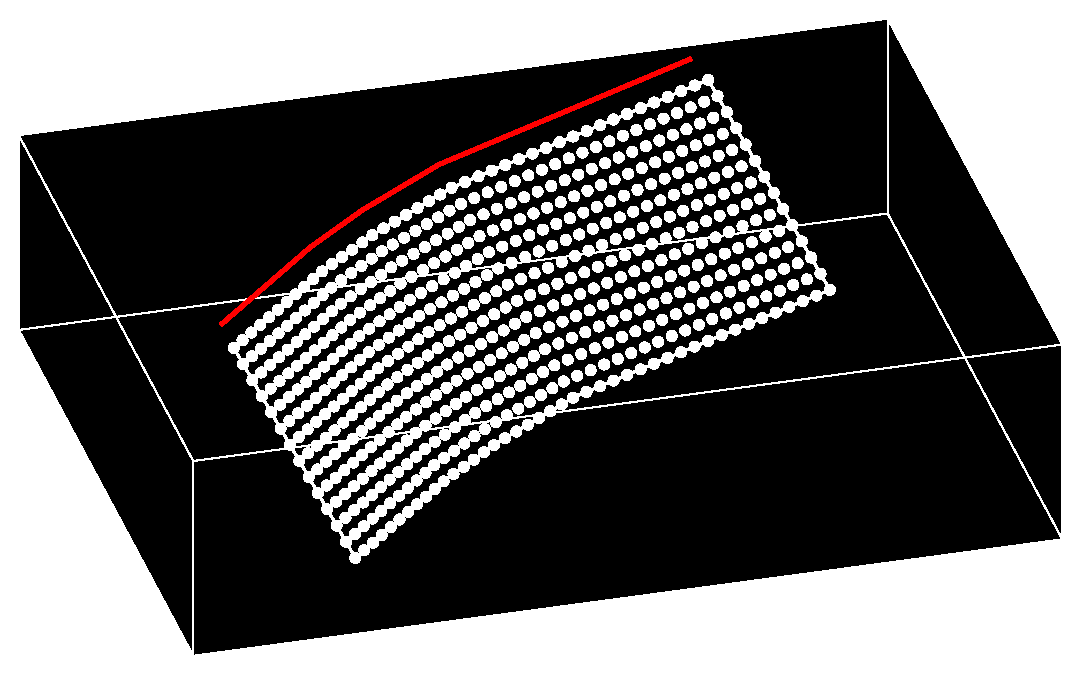
\includegraphics[width=5cm]{./oqum_Figures/simpleFaultMesh.eps}}
\subfigure[]{
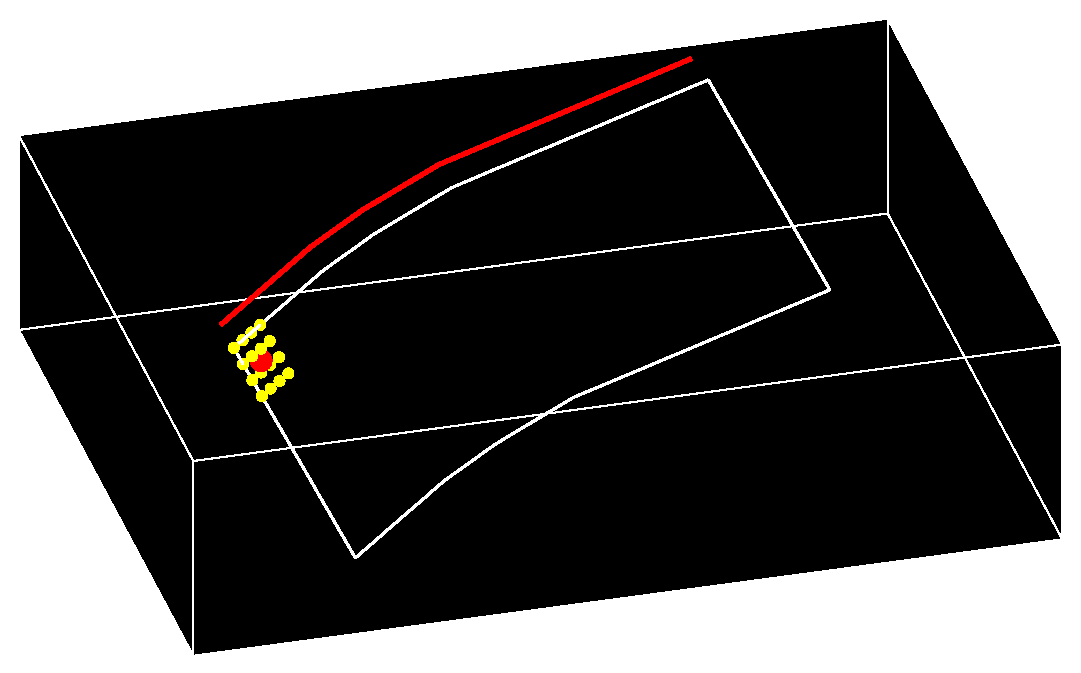
\includegraphics[width=5cm]{./oqum_Figures/simpleFaultMag5.eps}}
\subfigure[]{
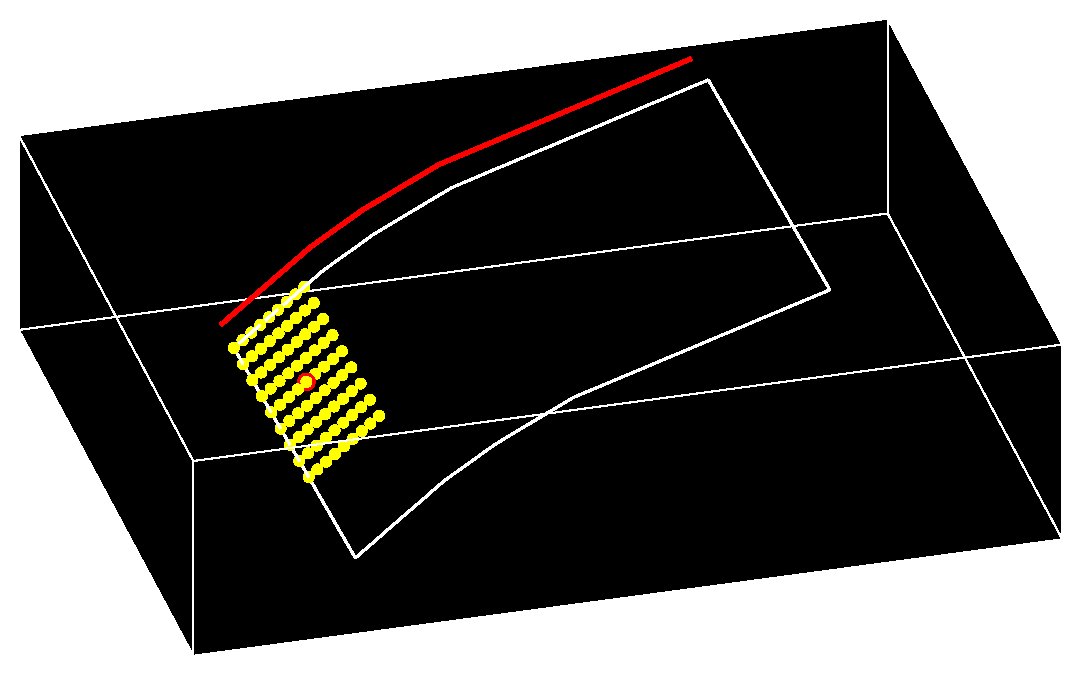
\includegraphics[width=5cm]{./oqum_Figures/simpleFaultMag6.eps}}
\caption{Fault rupture modeling. The fault surface is modeled by a regular mesh (a). Ruptures are modeled as portions of the fault surface mesh. Rupture dimensions (derived from magnitude using scaling relationship and aspect ratio) determine how many grid points are included in each rupture. Examples of ruptures of magnitude 5 (b) and 6 (c) are shown (assuming an aspect ration equal to 1). The red dot represent the hypocenter location.}
\label{faultSurface}
\end{center}
\end{figure}
\begin{figure}[!htbp]
\begin{center}
\subfigure[]{
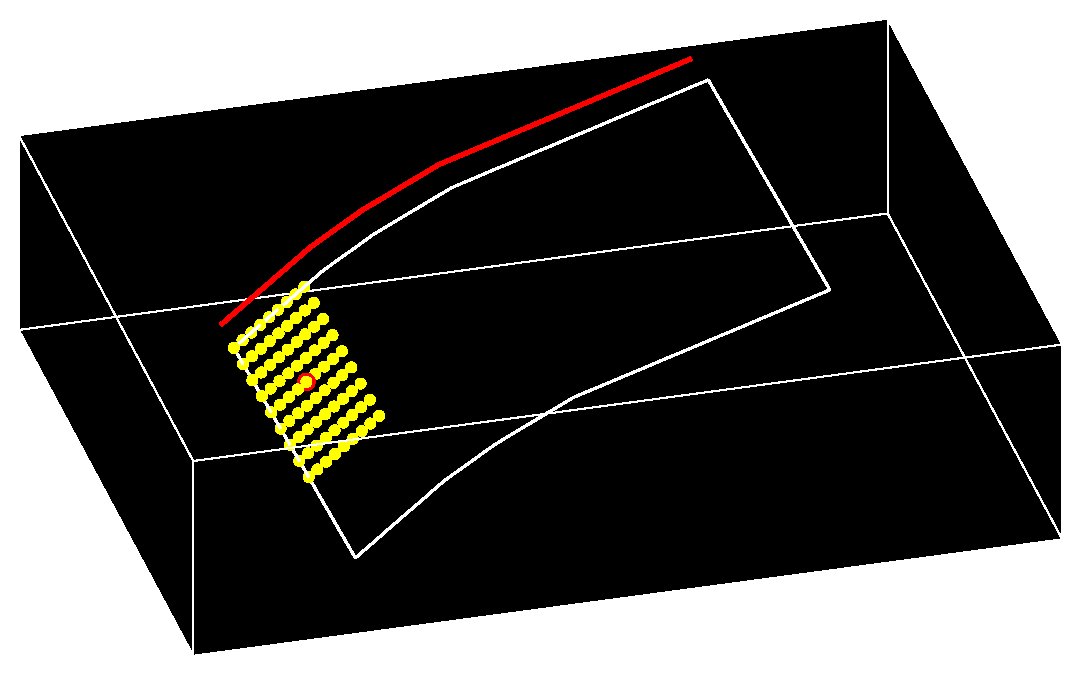
\includegraphics[width=5cm]{./oqum_Figures/simpleFaultMag6.eps}}
\subfigure[]{
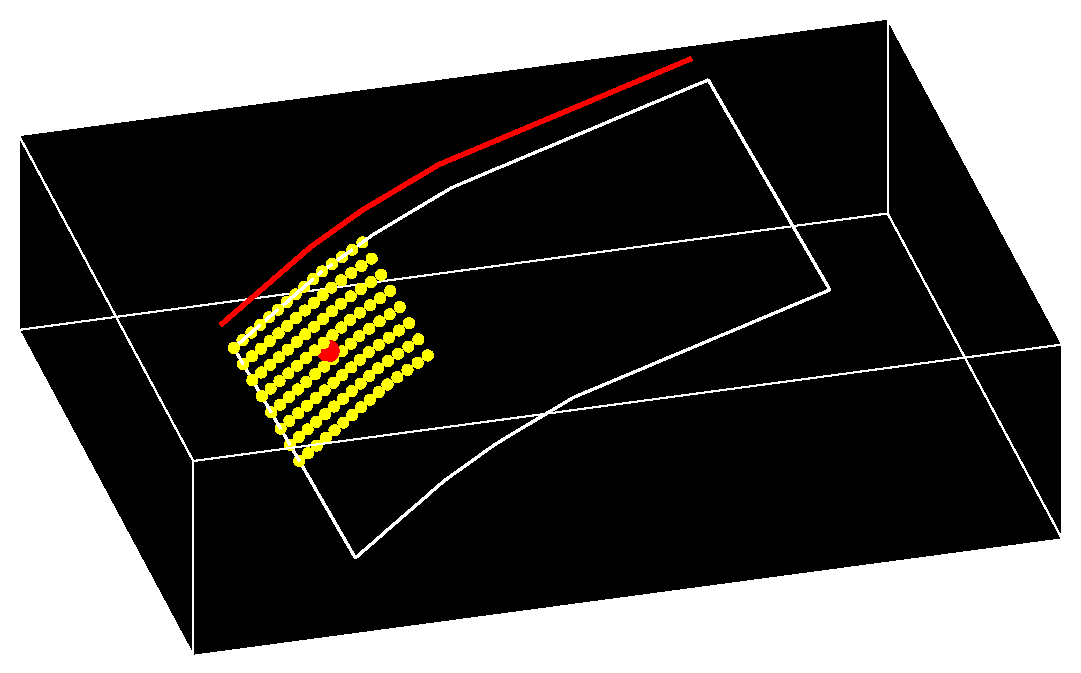
\includegraphics[width=5cm]{./oqum_Figures/simpleFaultMag6AR2.eps}}
\subfigure[]{
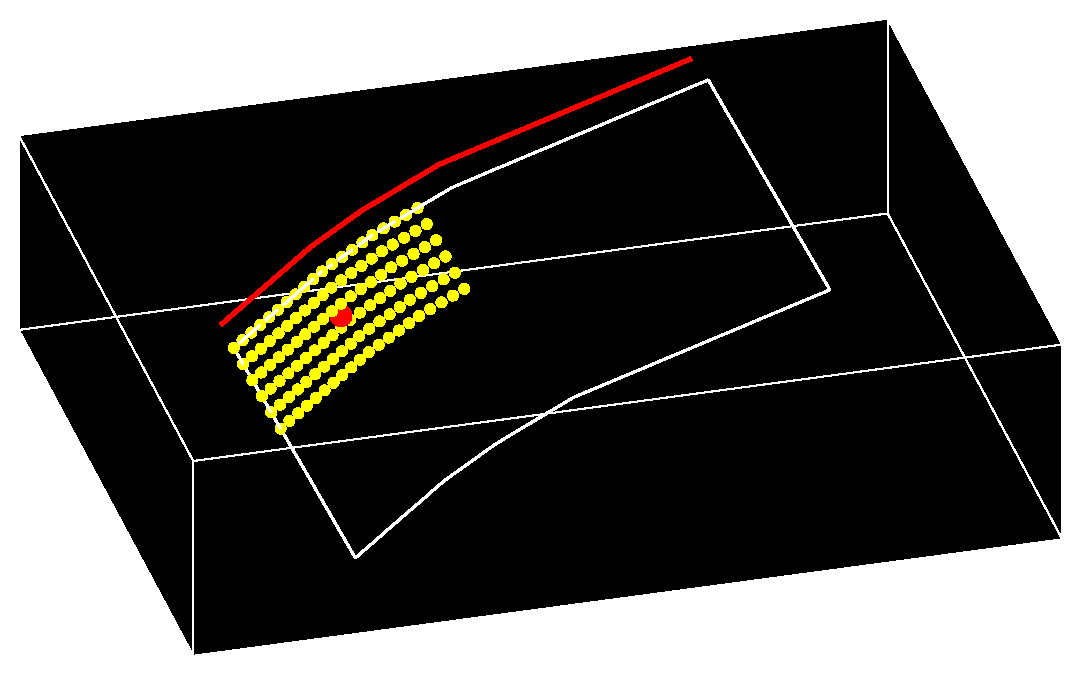
\includegraphics[width=5cm]{./oqum_Figures/simpleFaultMag6AR4.eps}}
\caption{Rupture modeling with magnitude-area scaling relationship. For the same magnitude (6 in this case), different aspect ratios [1 (a), 2, (b), 4 (c)]  produce ruptures with different lengths/widths but having the same area.}
\label{aspectRationMagArea}
\end{center}
\end{figure}
\begin{figure}[!htbp]
\begin{center}
\subfigure[]{
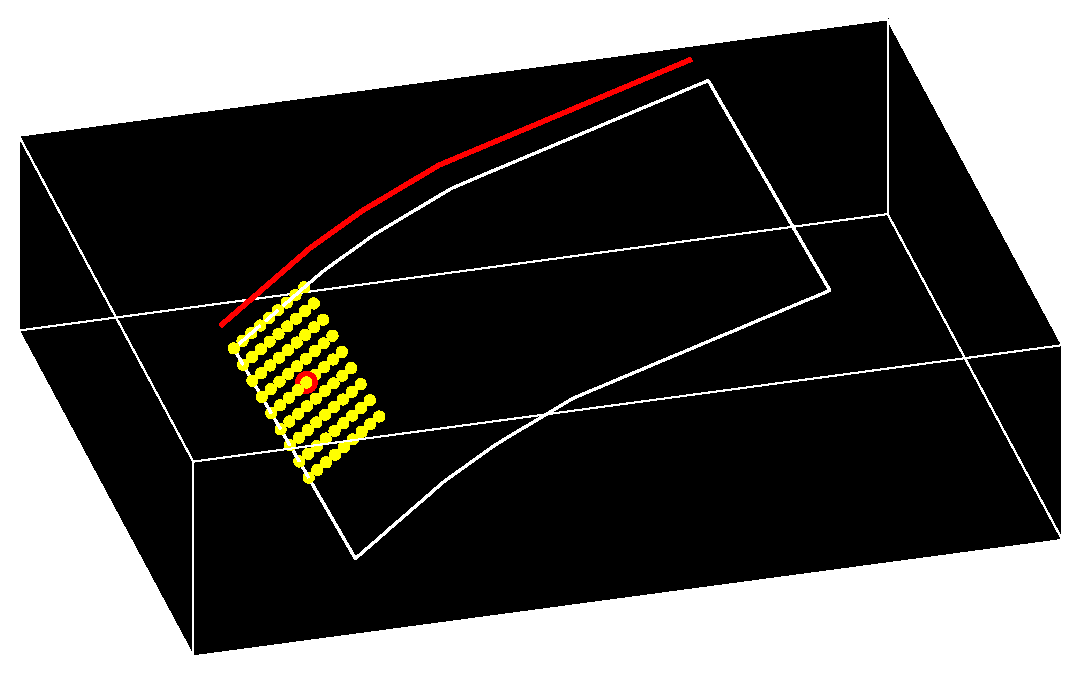
\includegraphics[width=5cm]{./oqum_Figures/simpleFaultMag6MagLengthRel.eps}}
\subfigure[]{
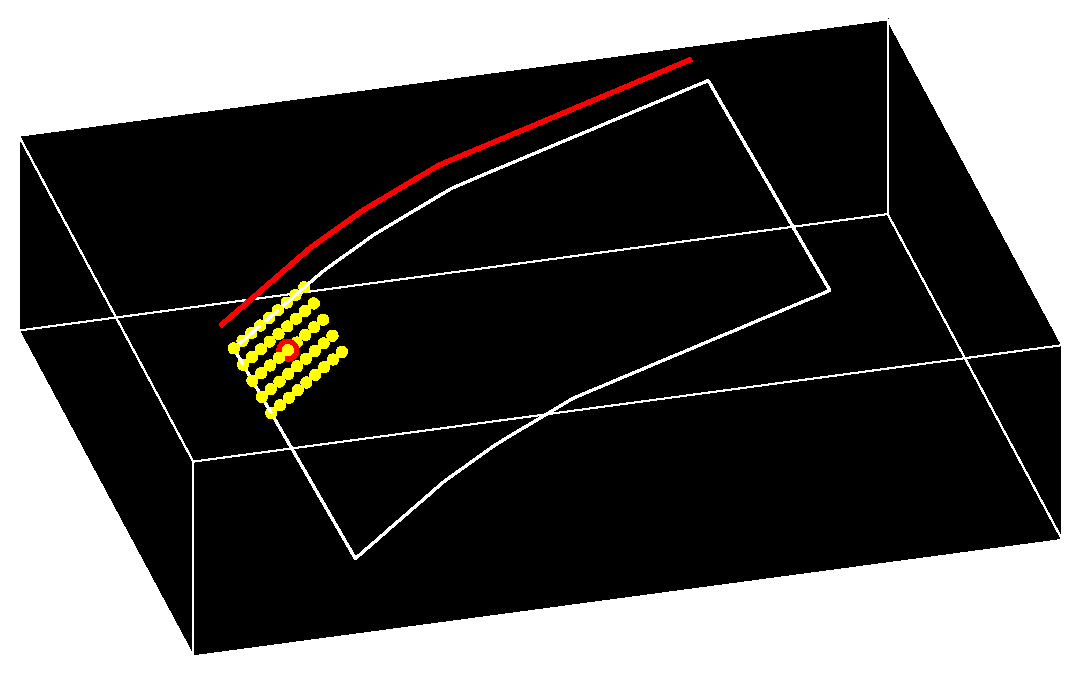
\includegraphics[width=5cm]{./oqum_Figures/simpleFaultMag6AR2MagLengthRel.eps}}
\subfigure[]{
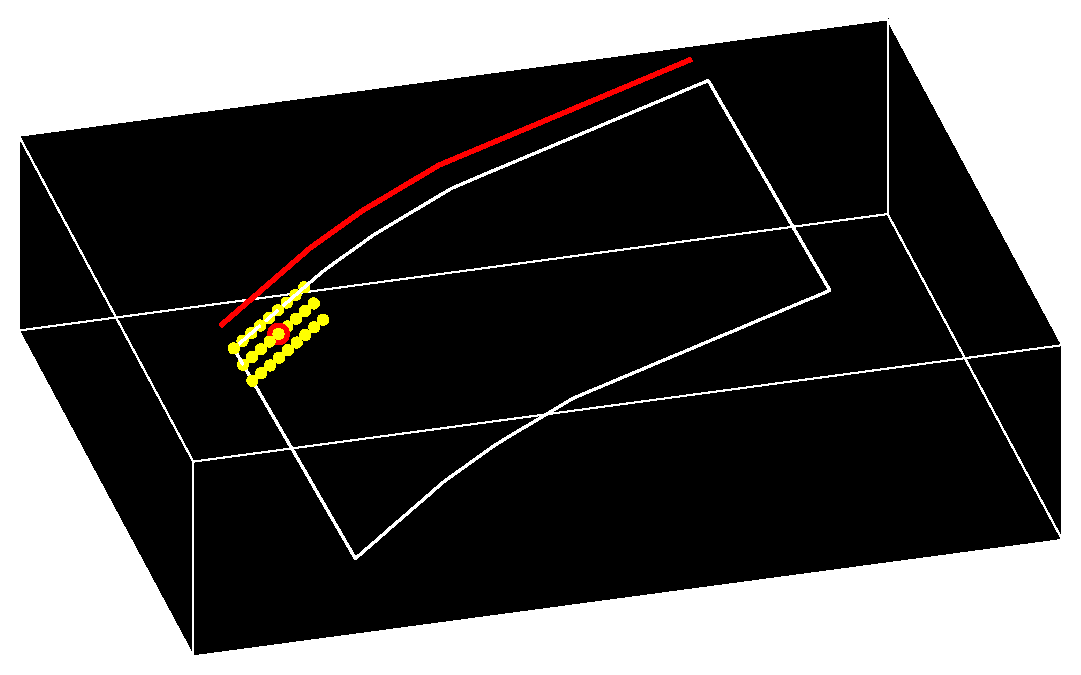
\includegraphics[width=5cm]{./oqum_Figures/simpleFaultMag6AR4MagLengthRel.eps}}
\caption{Rupture modeling with magnitude-length scaling relationship. For the same magnitude (6 in this case), different aspect ratios [1 (a), 2, (b), 4 (c)]  produce ruptures with same lengths, but different widths, associated therefore to different areas.}
\label{aspectRationMagLength}
\end{center}
\end{figure}
\begin{figure}[!htbp]
\begin{center}
\subfigure[]{
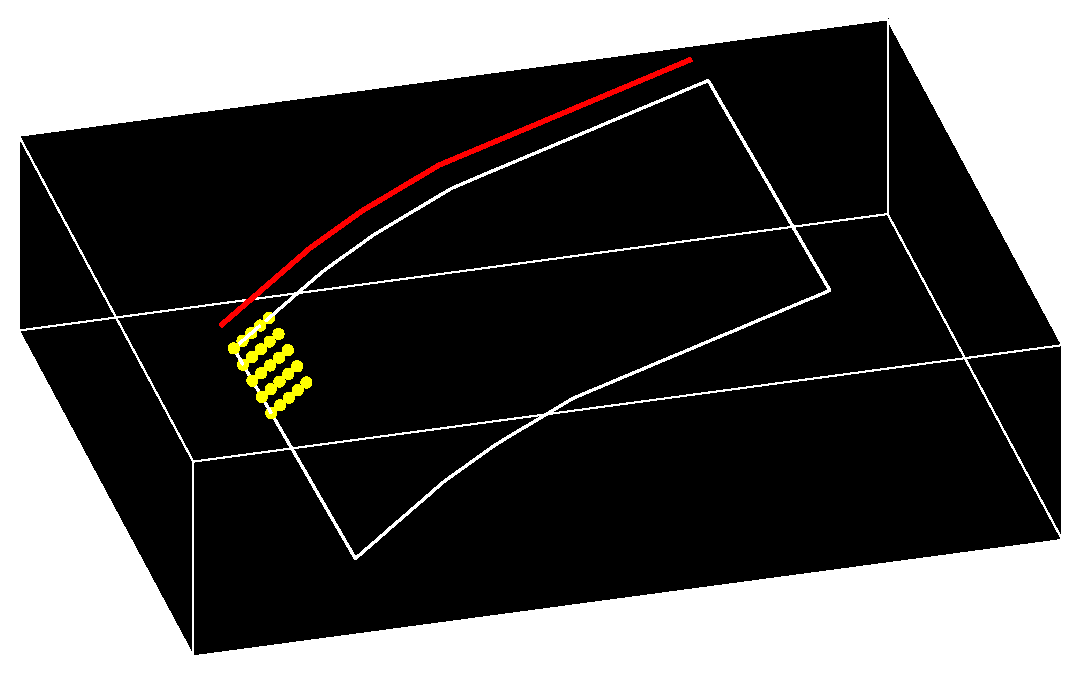
\includegraphics[width=4cm]{./oqum_Figures/mag6_1.eps}}
\subfigure[]{
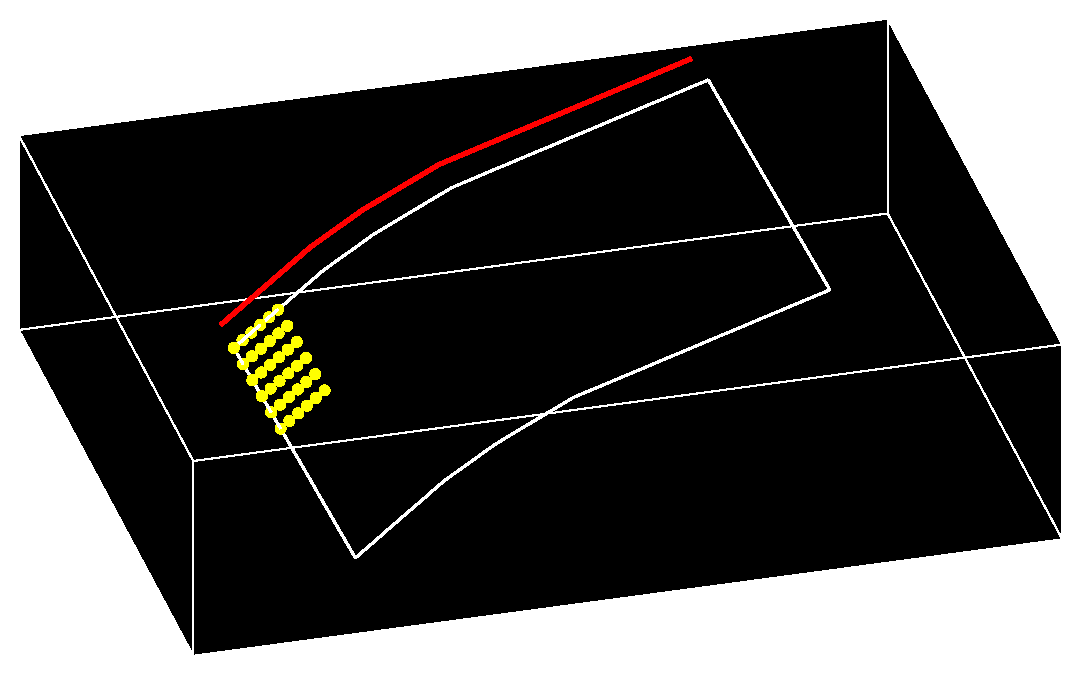
\includegraphics[width=4cm]{./oqum_Figures/mag6_2.eps}}
\subfigure[]{
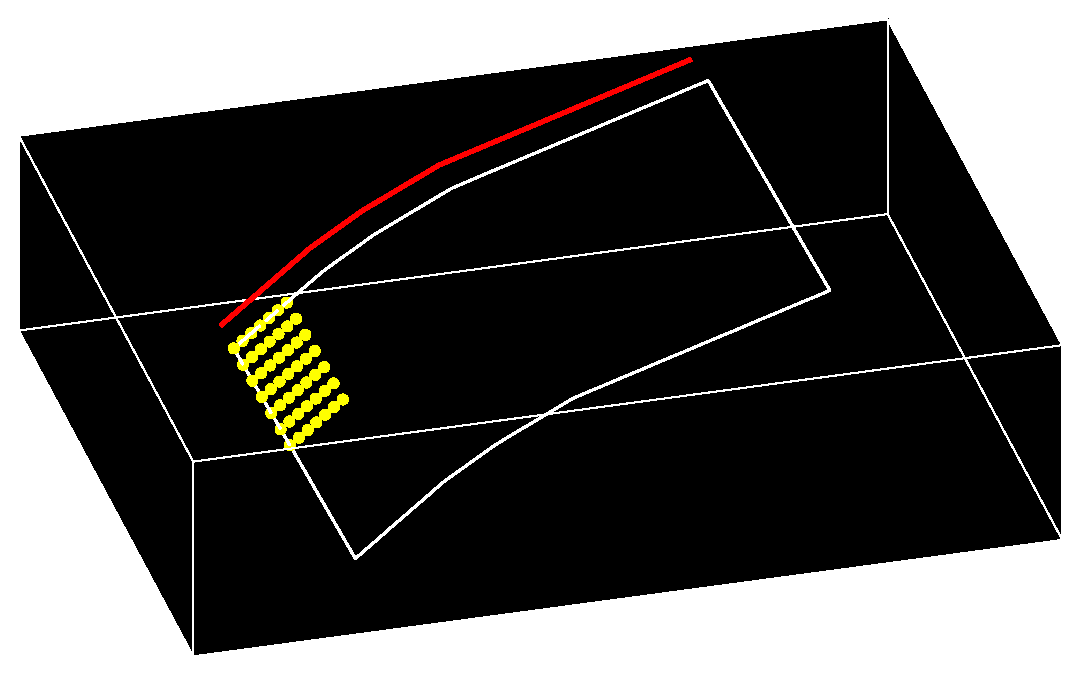
\includegraphics[width=4cm]{./oqum_Figures/mag6_3.eps}}
\subfigure[]{
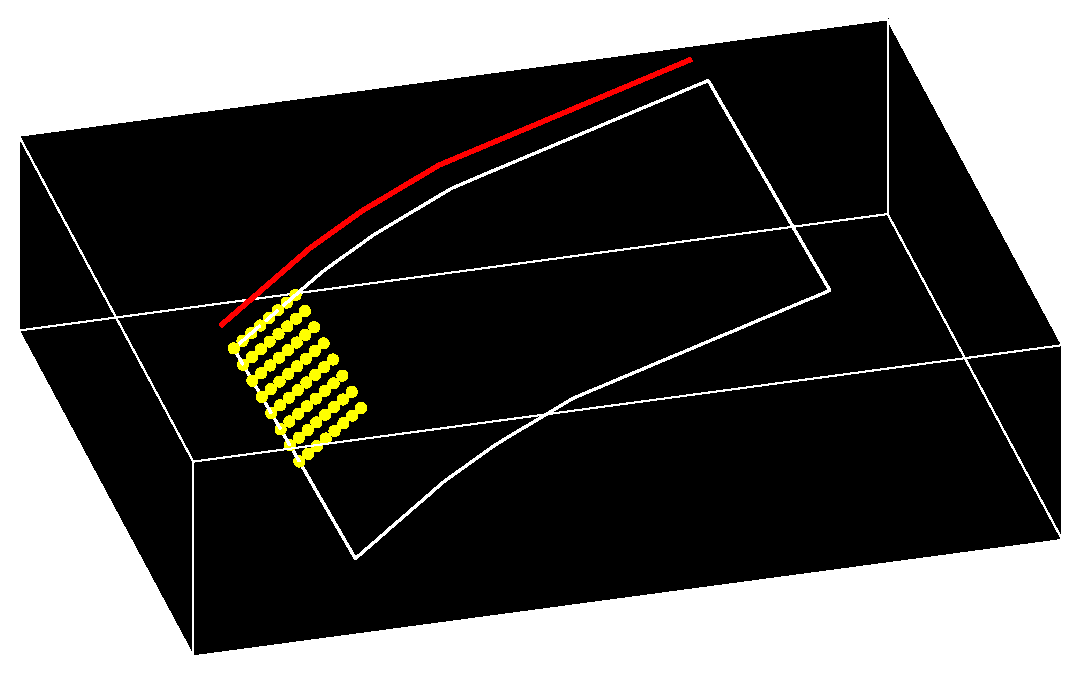
\includegraphics[width=4cm]{./oqum_Figures/mag6_4.eps}}
\subfigure[]{
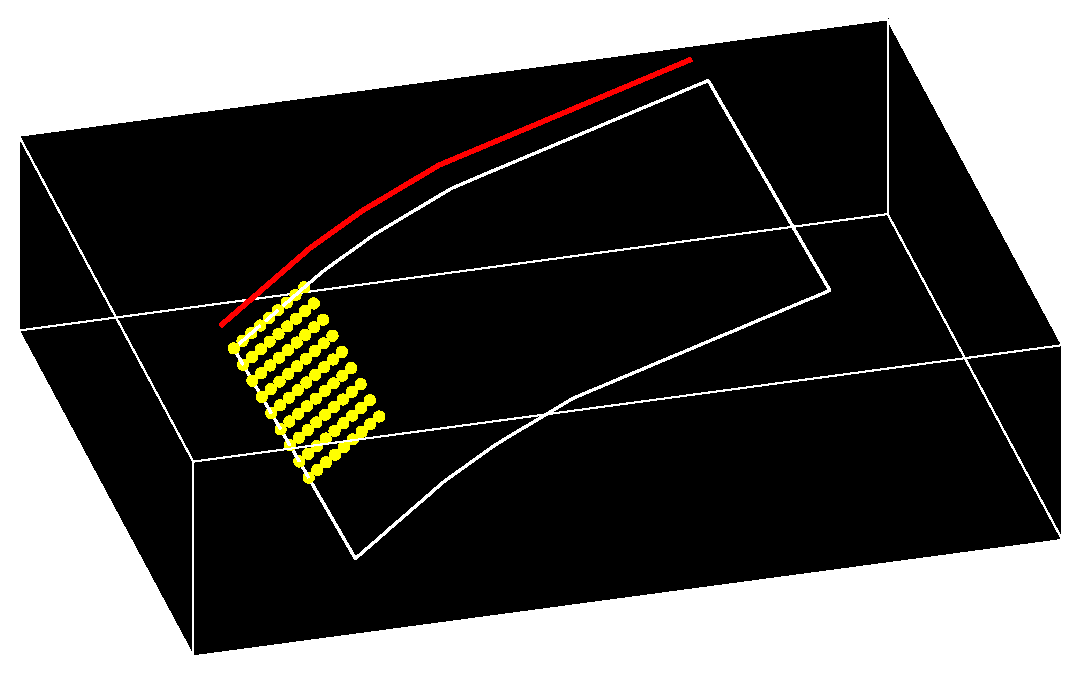
\includegraphics[width=4cm]{./oqum_Figures/mag6_5.eps}}
\subfigure[]{
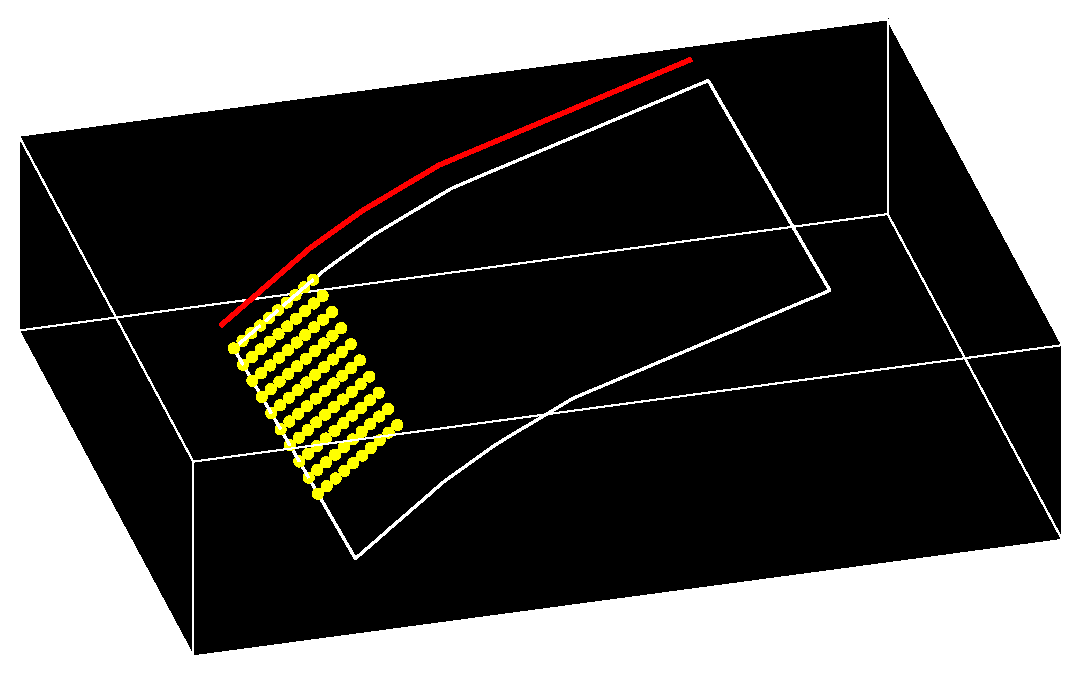
\includegraphics[width=4cm]{./oqum_Figures/mag6_6.eps}}
\subfigure[]{
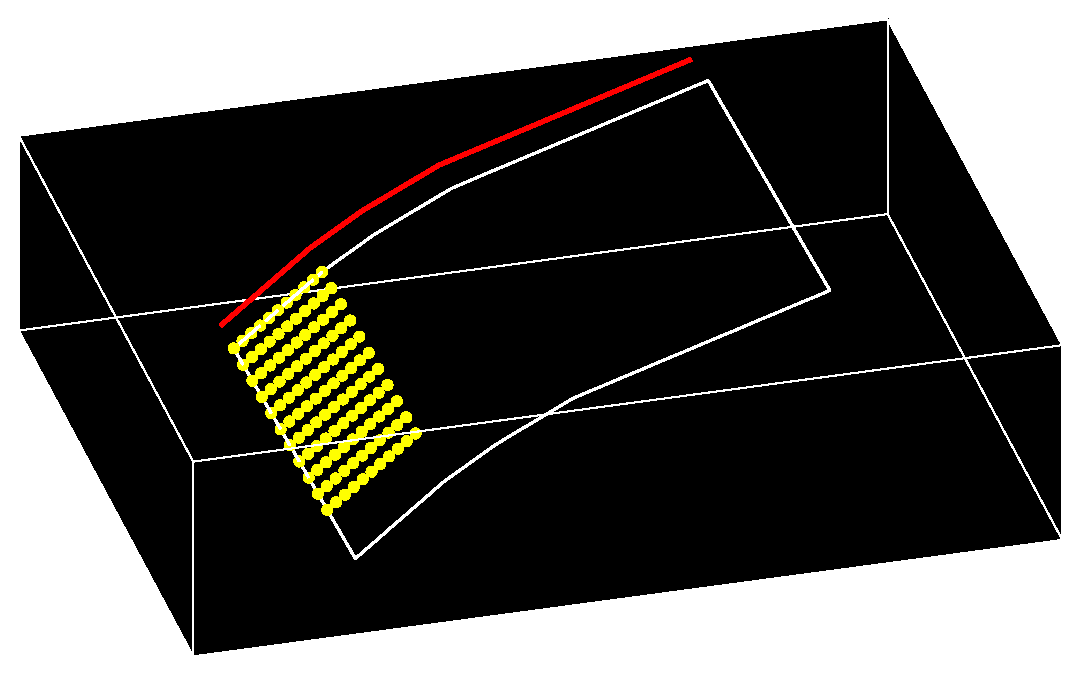
\includegraphics[width=4cm]{./oqum_Figures/mag6_7.eps}}
\subfigure[]{
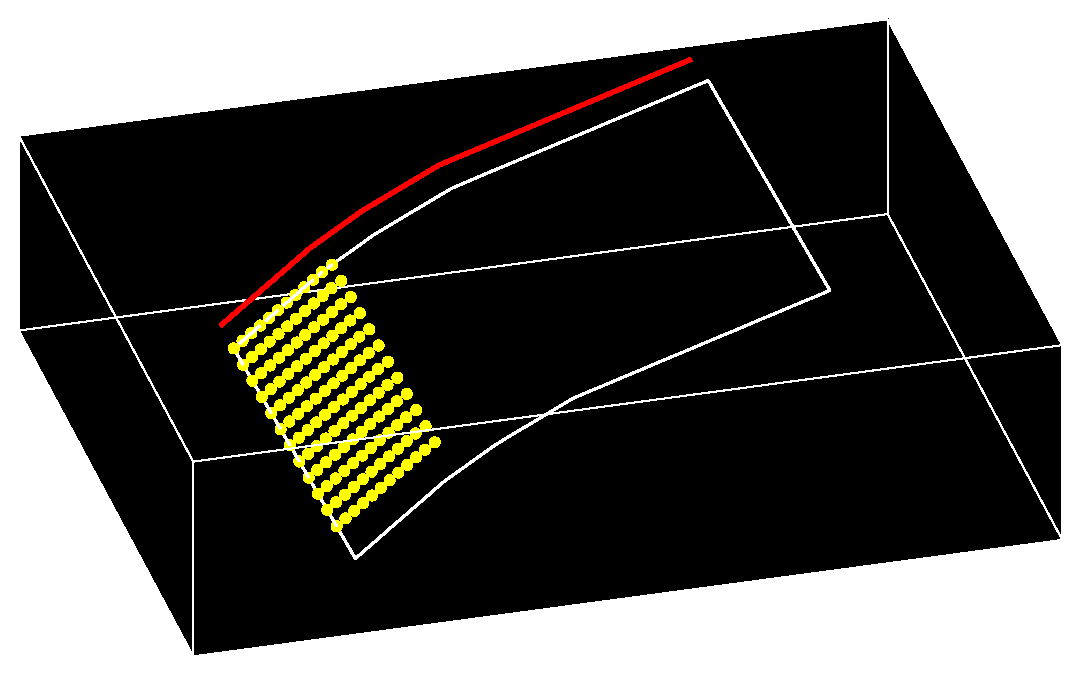
\includegraphics[width=4cm]{./oqum_Figures/mag6_8.eps}}
\subfigure[]{
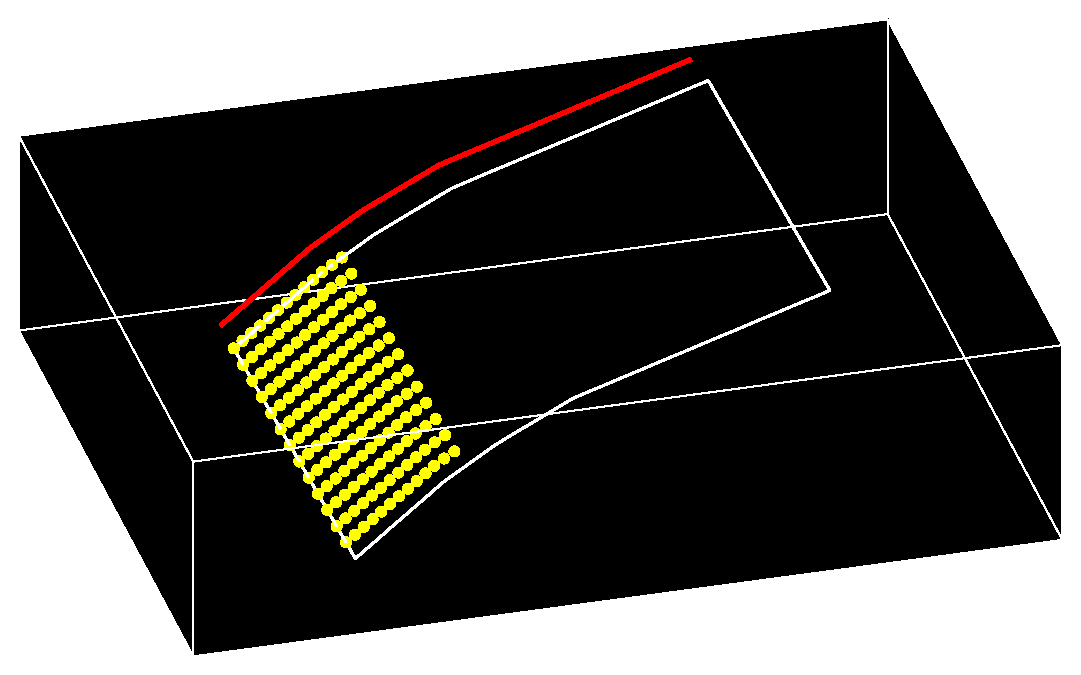
\includegraphics[width=4cm]{./oqum_Figures/mag6_9.eps}}
\subfigure[]{
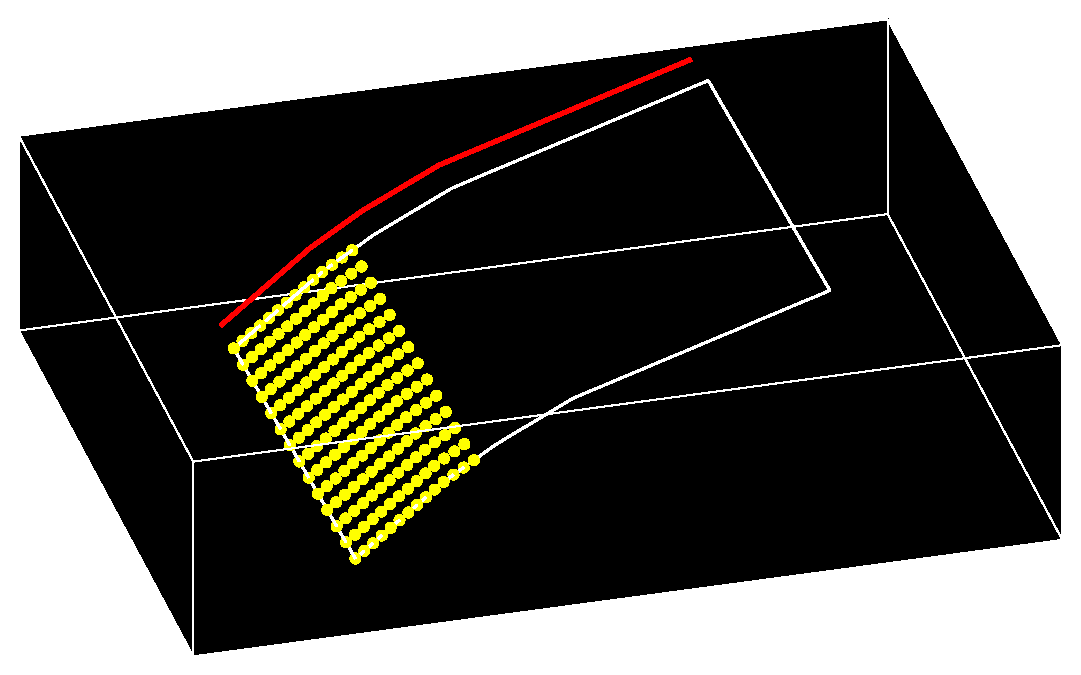
\includegraphics[width=4cm]{./oqum_Figures/mag6_10.eps}}
\subfigure[]{
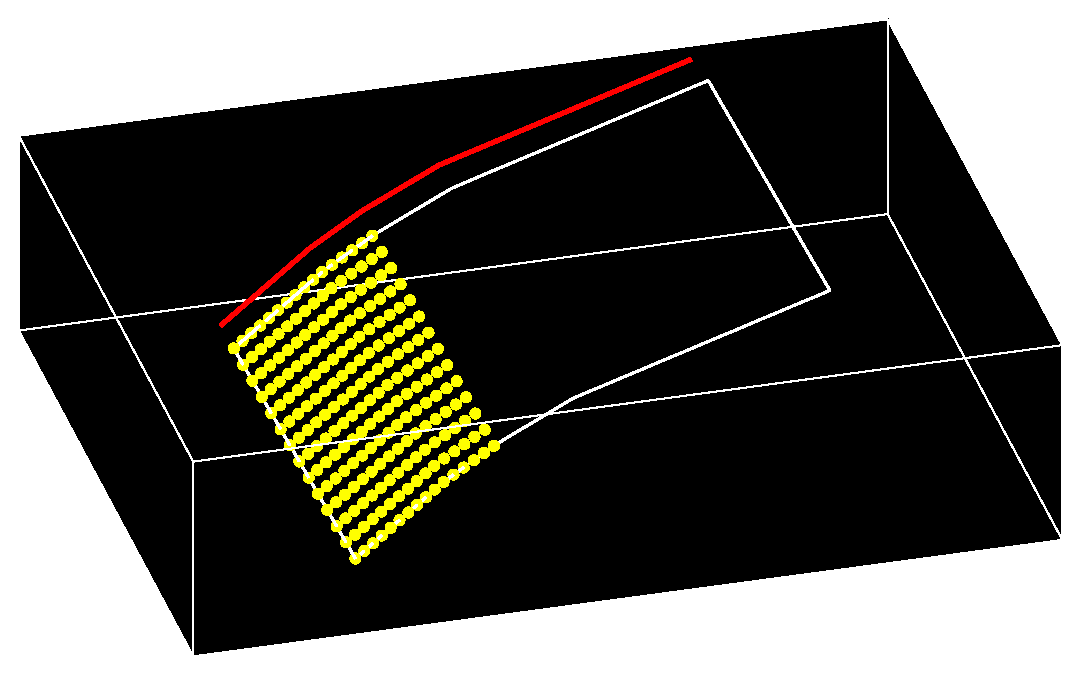
\includegraphics[width=4cm]{./oqum_Figures/mag6_11.eps}}
\subfigure[]{
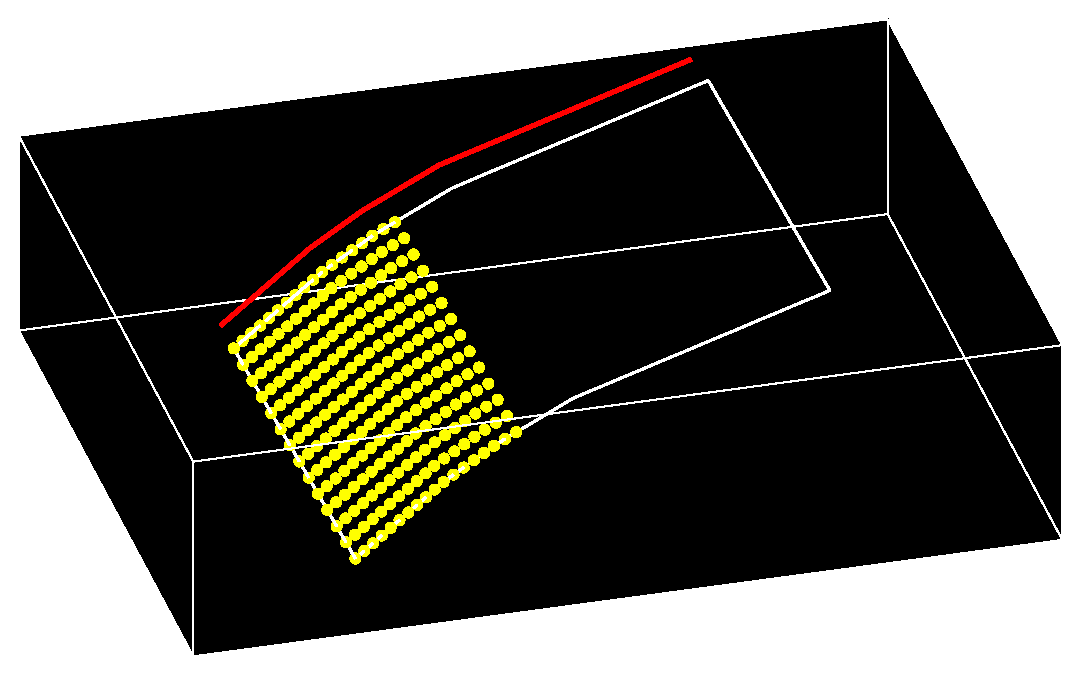
\includegraphics[width=4cm]{./oqum_Figures/mag6_12.eps}}
\subfigure[]{
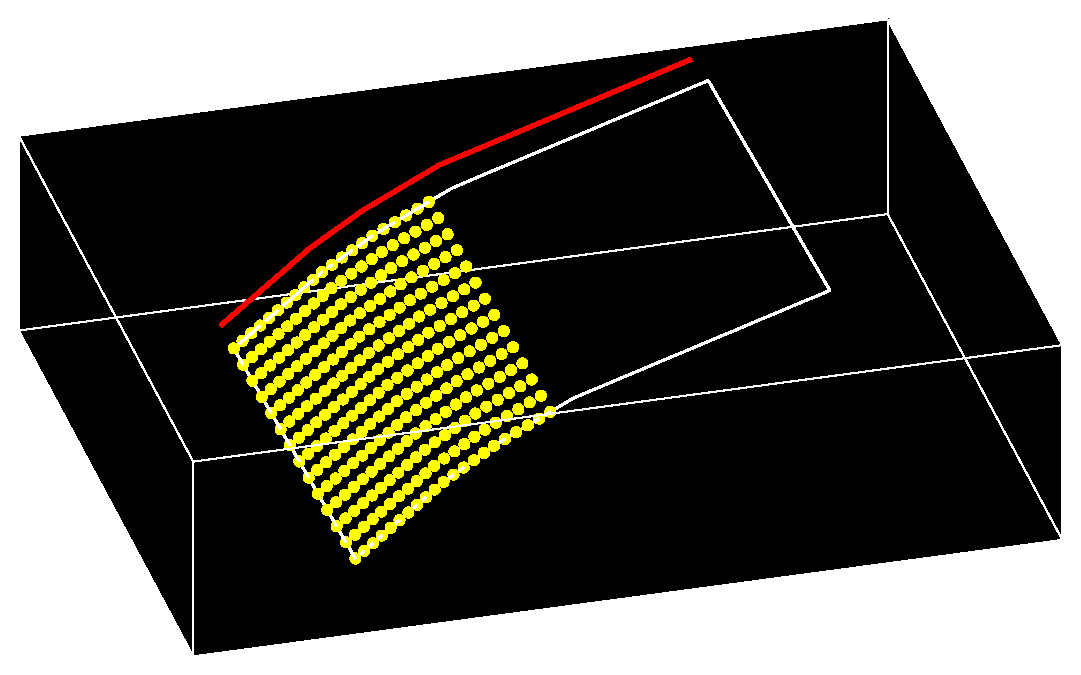
\includegraphics[width=4cm]{./oqum_Figures/mag6_13.eps}}
\subfigure[]{
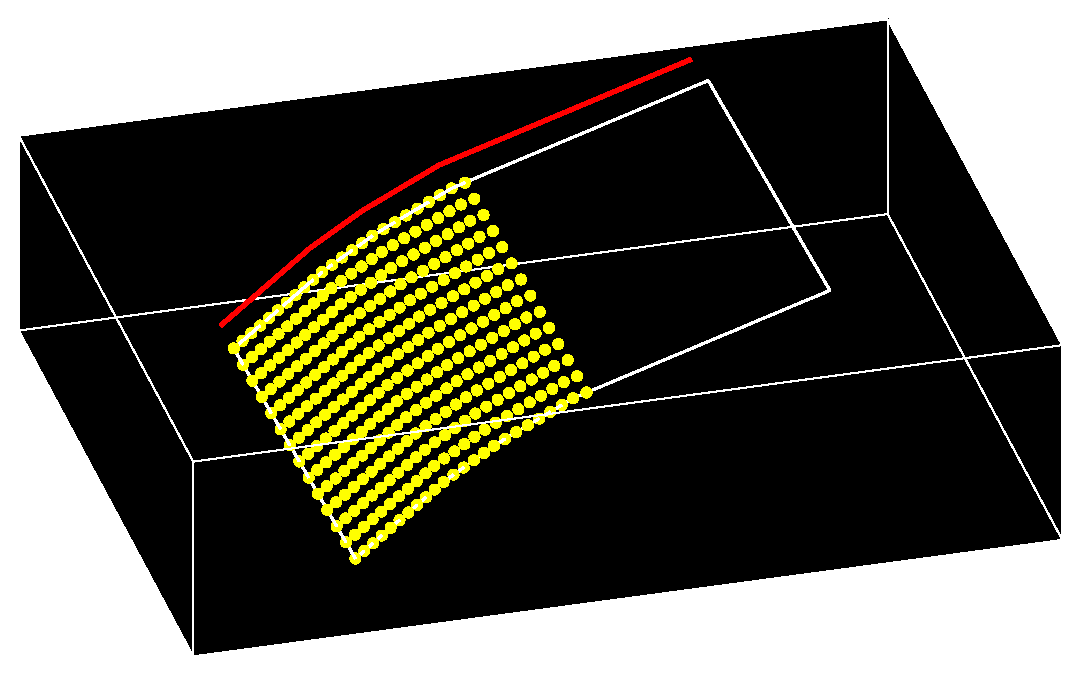
\includegraphics[width=4cm]{./oqum_Figures/mag6_14.eps}}
\subfigure[]{
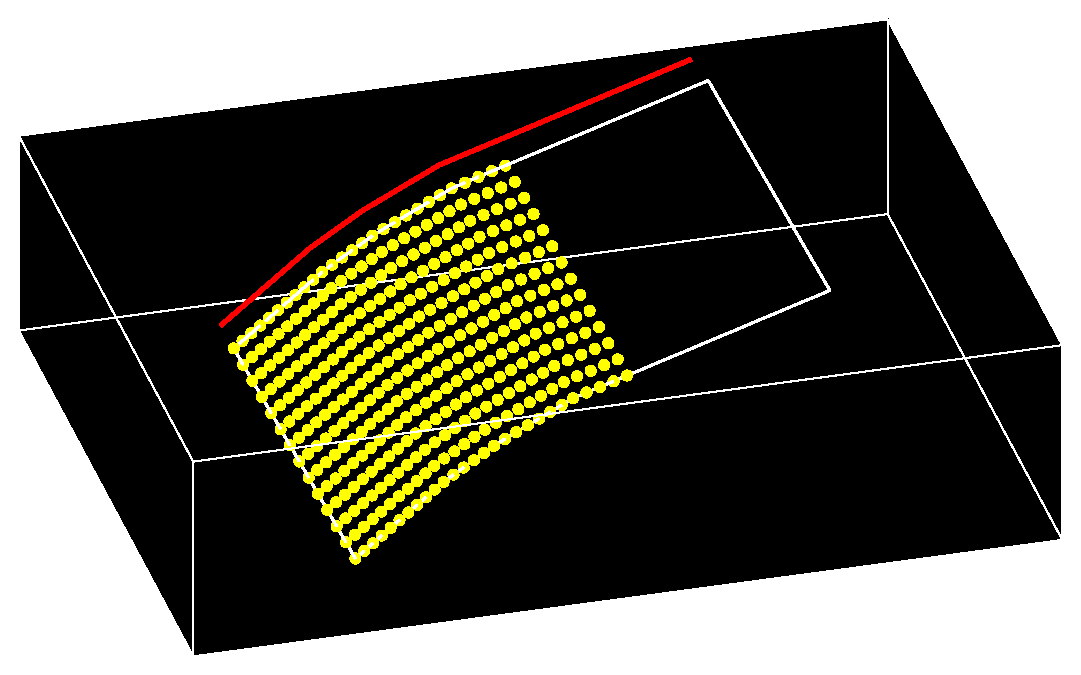
\includegraphics[width=4cm]{./oqum_Figures/mag6_15.eps}}
\subfigure[]{
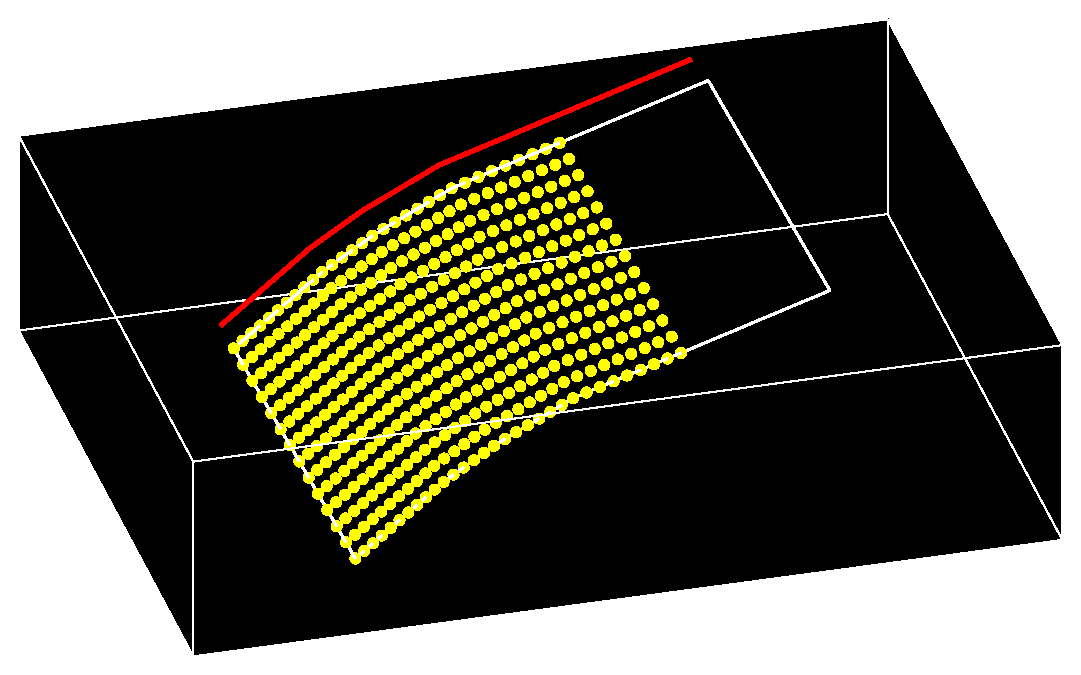
\includegraphics[width=4cm]{./oqum_Figures/mag6_16.eps}}
\subfigure[]{
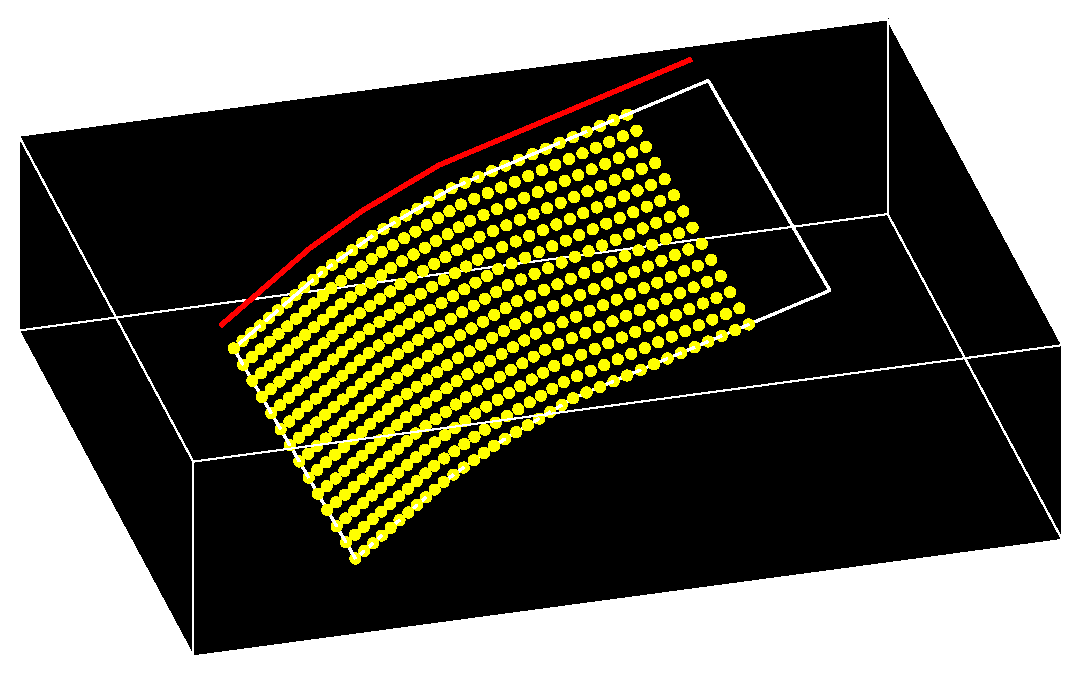
\includegraphics[width=4cm]{./oqum_Figures/mag6_17.eps}}
\subfigure[]{
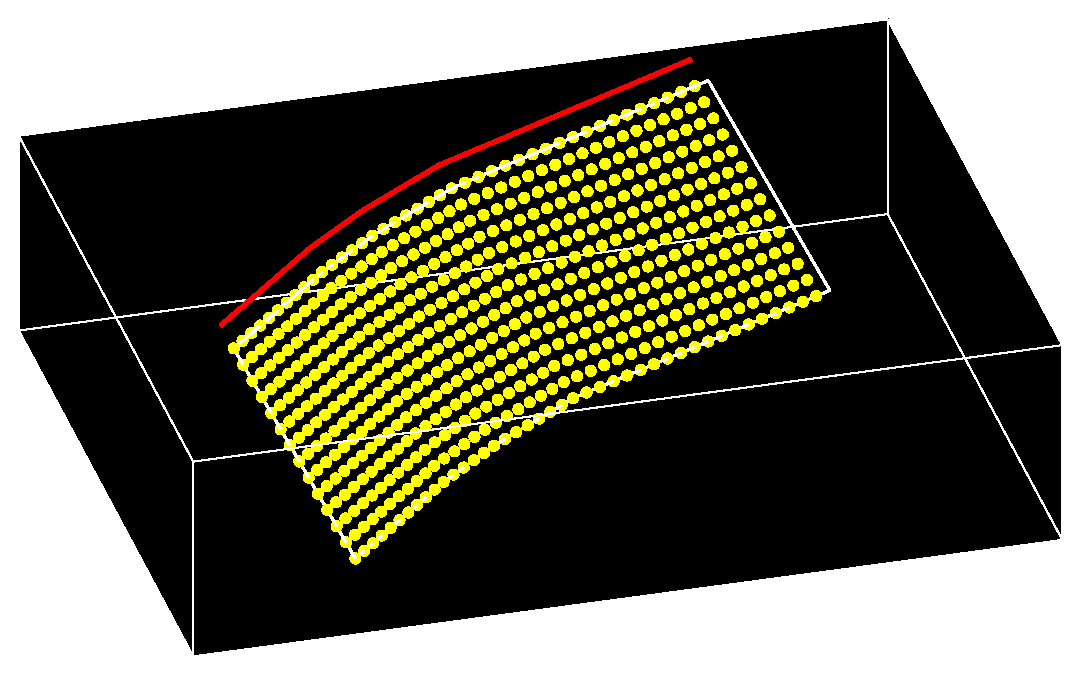
\includegraphics[width=4cm]{./oqum_Figures/mag6_18.eps}}
\caption{Uncertainties in scaling relationship. For the same position on the fault (fault's upper left corner), for the same magnitude (in this case 6), multiple ruptures are generated but with different areas (in this examples ruptures are generate using a magnitude area scaling relationship with standard deviation set to 0.25).}
\label{scalingSigma}
\end{center}
\end{figure}
\begin{figure}[!htbp]
\begin{center}
\subfigure[]{
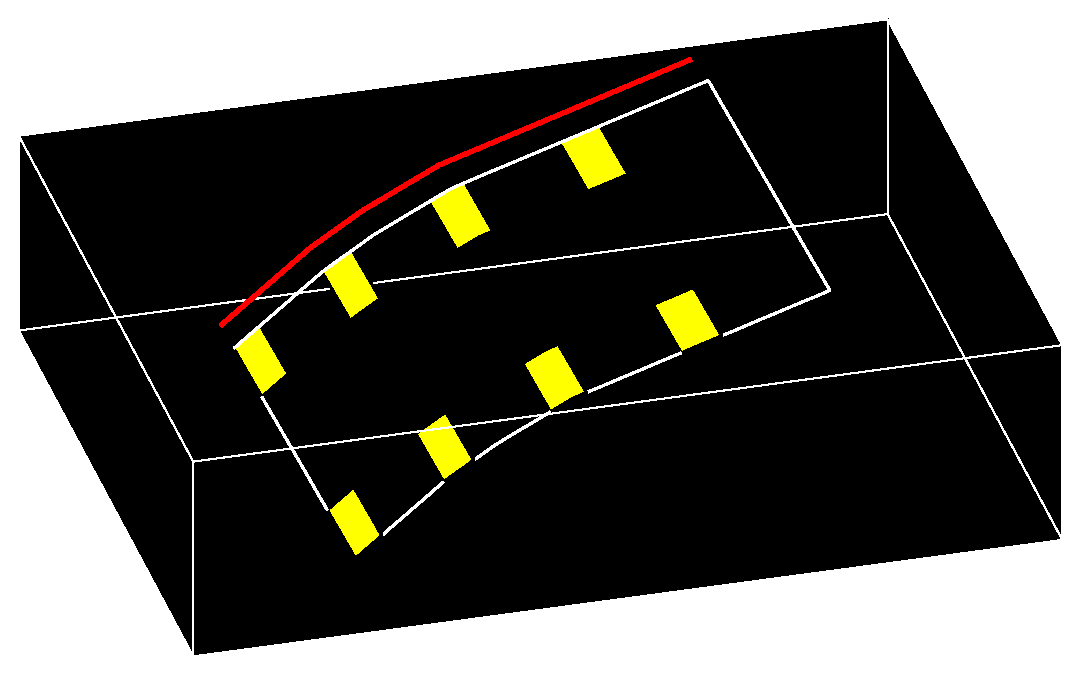
\includegraphics[width=5cm]{./oqum_Figures/ruptFloatingMag5OffSet10km.eps}}
\subfigure[]{
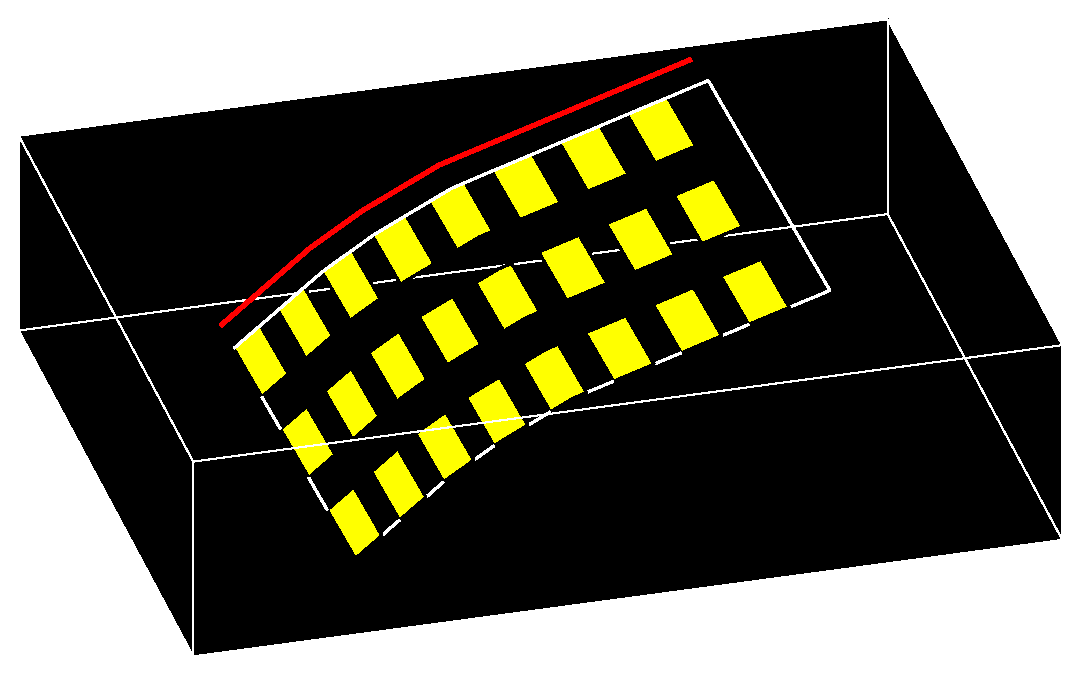
\includegraphics[width=5cm]{./oqum_Figures/ruptFloatingMag5OffSet5km.eps}}
\subfigure[]{
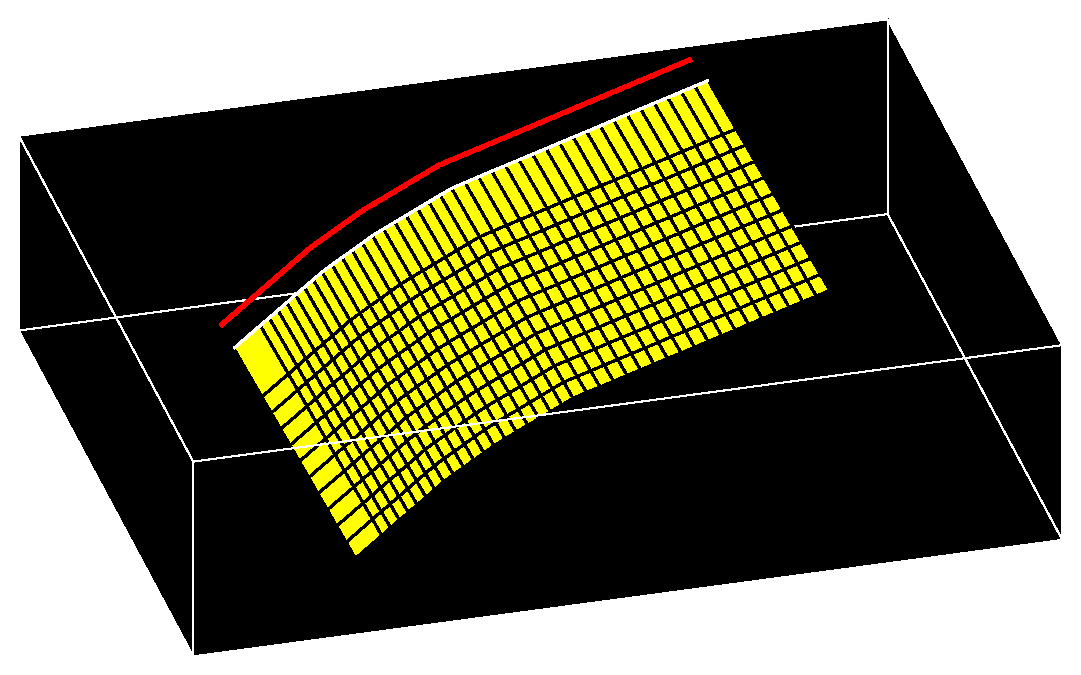
\includegraphics[width=5cm]{./oqum_Figures/ruptFloatingMag5OffSet1km.eps}}
\caption{The rupture offset. By decreasing the rupture offset (10 km (a), 5 km (b), 1 km (c)), earthquake ruptures can better cover the fault surface.}
\label{ruptureOffSet}
\end{center}
\end{figure}
\begin{figure}[!htbp]
\begin{center}
\subfigure[]{
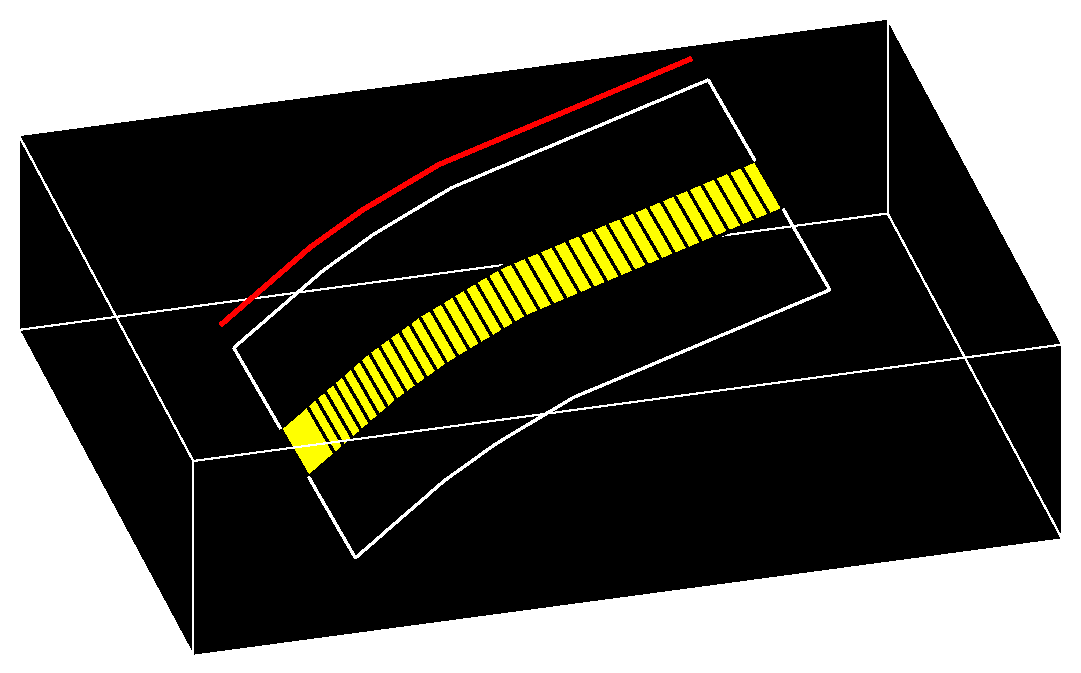
\includegraphics[width=5cm]{./oqum_Figures/ruptFloatingCentered.eps}}
\subfigure[]{
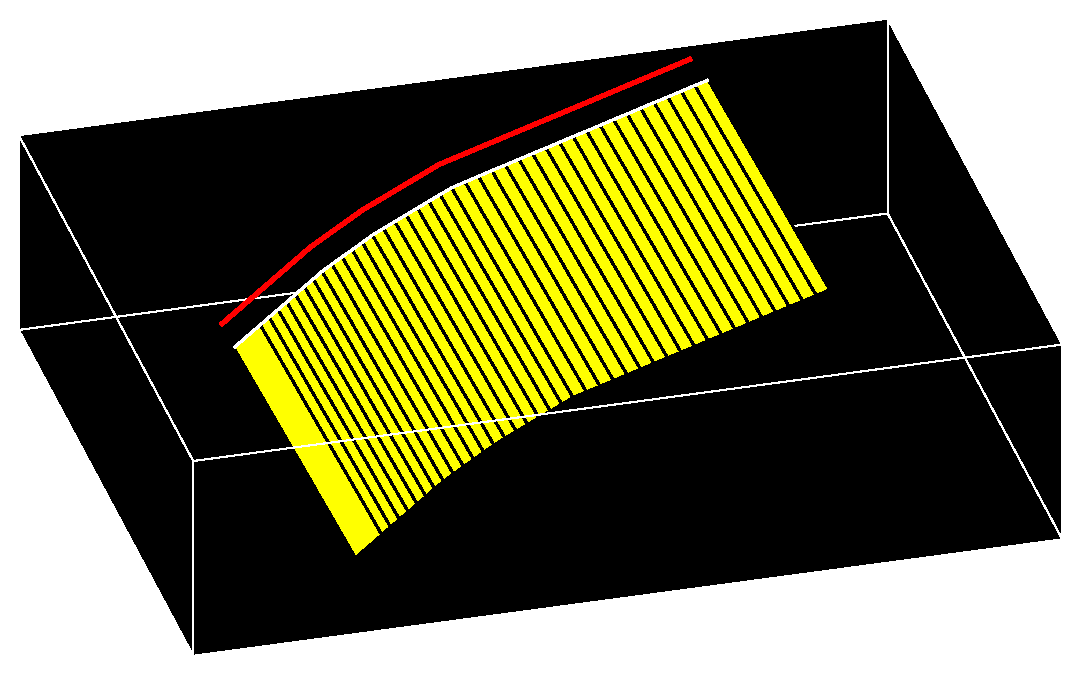
\includegraphics[width=5cm]{./oqum_Figures/ruptFloatingFullDDW.eps}}
\subfigure[]{
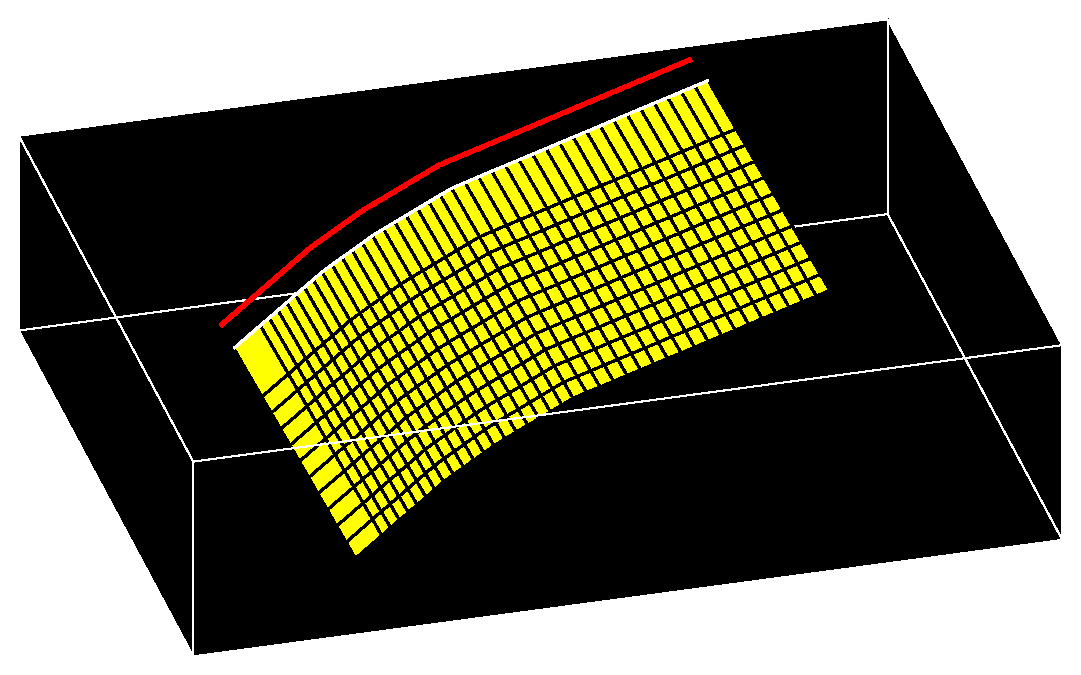
\includegraphics[width=5cm]{./oqum_Figures/ruptFloatingMag5OffSet1km.eps}}
\caption{Options for rupture floating. Rupture floating only along strike but centered along dip (a) or along strike and extending ruptures fully along dip (b), or along strike and along dip (c).}
\label{ruptureFloating}
\end{center}
\end{figure}

\subsubsection{Complex Fault source parameters}
Complex fault sources require the same set of parameters of simple fault sources:
\begin{itemize}
\item \Verb+INCLUDE_SUBDUCTION_FAULT_SOURCE+: if \Verb+true+ all complex fault sources in the source model are included in the ERF calculation. They are exclude if \Verb+false+.
\item \Verb+SUBDUCTION_FAULT_SURFACE_DISCRETIZATION+:  specifies the fault surface discretization step (in km). Minimum value is 1 km (which can be considered a typical value too).
\item \Verb+SUBDUCTION_FAULT_MAGNITUDE_SCALING_RELATIONSHIP+:  specifies the magnitude scaling relationship used for modeling finite ruptures. It can be a magnitude-area or a magnitude-length relationship (list of available scaling relationships are given in Appendix B).
\item \Verb+SUBDUCTION_FAULT_MAGNITUDE_SCALING_SIGMA+: the standard deviation of log(Length) or log(Area). 0 if no uncertainties are considered.
\item \Verb+SUBDUCTION_RUPTURE_ASPECT_RATIO+: rupture aspect ratio (rupture length / rupture width). Determines the rupture shape (square if 1, rectangle elongated along strike if$ > 1$, or along dip if $< 1$).
\item \Verb+SUBDUCTION_FAULT_RUPTURE_OFFSET+: specifies the amount by which ruptures are offset on the fault (in km). It must be greater or equal to the fault surface discretization step. The rupture offset should be close to the dimensions of the minimum magnitude modeled on the fault to guarantee that the rupture distribution on the fault surface has no empty spaces.
\item \Verb+SUBDUCTION_RUPTURE_FLOATING_TYPE+: rupture floating algorithm. Allowed values are:
\begin{itemize}
\item \Verb+Only along strike ( rupture full DDW)+
\item \Verb+Along strike and down dip+
\item \Verb+Along strike & centered down dip+
\end{itemize}
\end{itemize}
A complex fault surface is modeled through a pseudo-regular mesh (Figure \ref{complexFault} (a)), that is mesh with a grid spacing that is not uniform but vary depending on the position on the surface. The actual surface discretization is 'approximately' equal to the specified surface discretization. In other words, the grid spacing in the actual mesh fluctuates around the specified surface discretization value. The intensity of these fluctuations depends on the degree of complexity of the surface geometry. Higher is the geometrical complexity, larger is the difference between the actual and specified grid spacing. As in a simple fault, ruptures are defined (by using scaling relationship and aspect ratio) as portions of the fault surface mesh (Figure \ref{complexFault} (b)). Rupture dimensions are computed with respect to the specified discretization step. If the difference between specified and actual grid spacing is large, the rupture dimensions, as modeled on the mesh, may not be exactly the same of the dimensions predicted by the scaling relationship. However, apart from the modeling of the fault surface mesh, rupture creation and floating is governed exactly in the same way as for simple faults and have the same options.\\
\begin{figure}[!htbp]
\begin{center}
\subfigure[]{
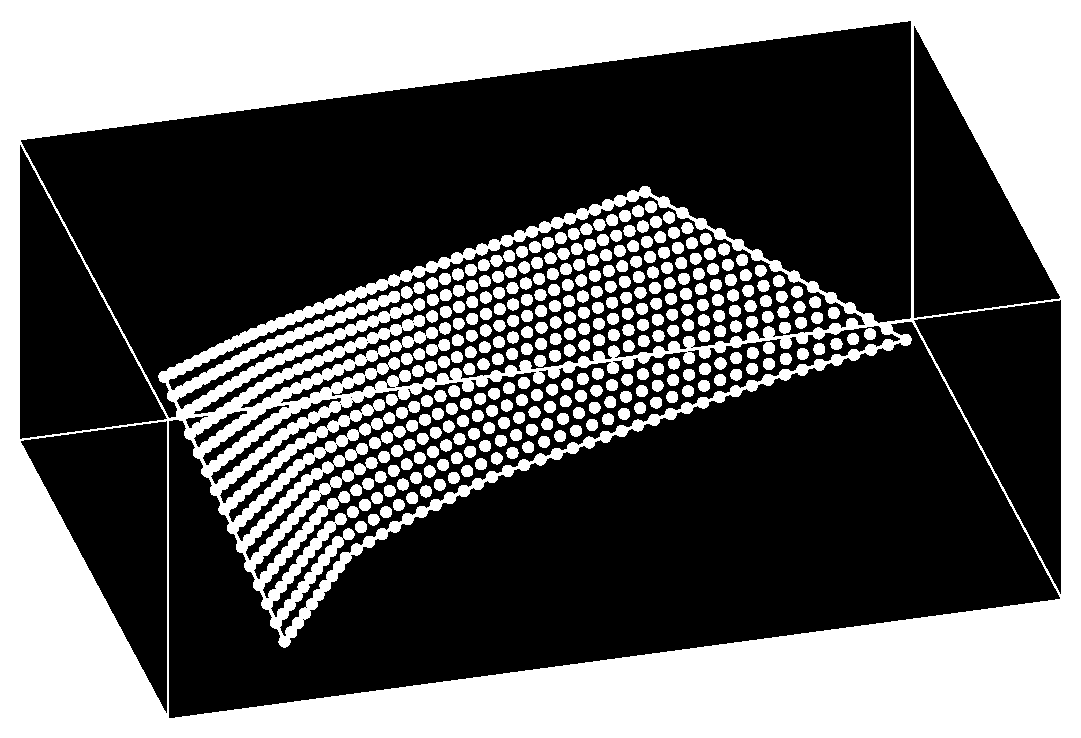
\includegraphics[width=5cm]{./oqum_Figures/complexFaultMesh.eps}}
\subfigure[]{
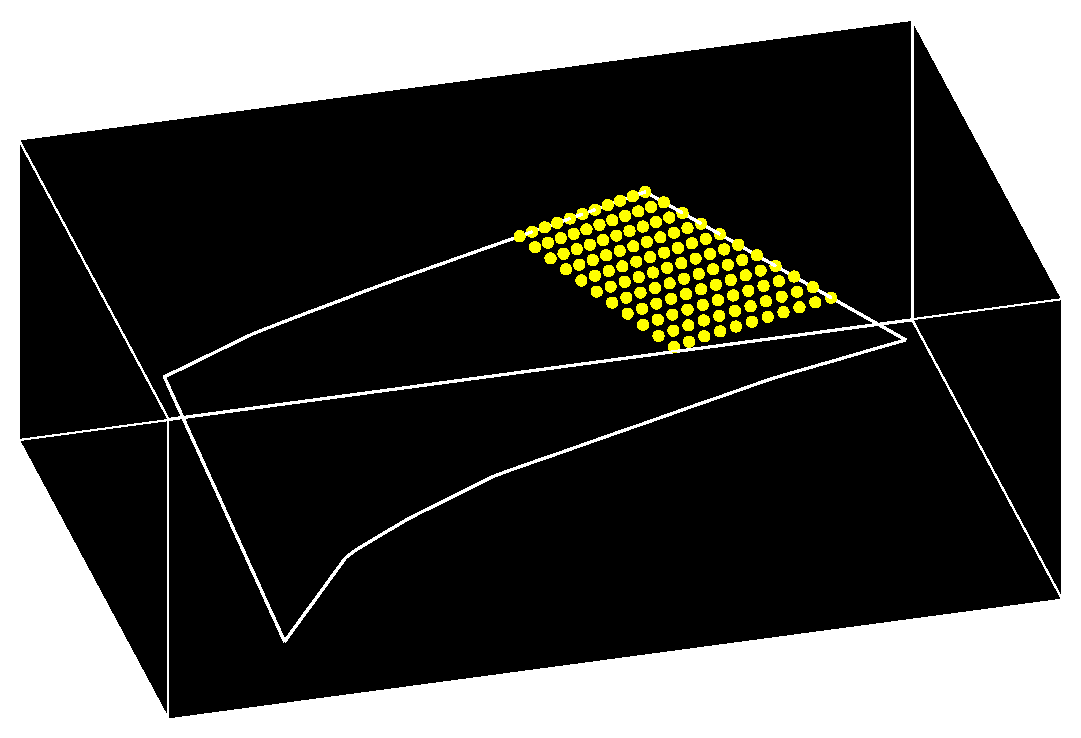
\includegraphics[width=5cm]{./oqum_Figures/complexFaultRupMag6.eps}}
\caption{Complex fault modeling. From the top and bottom fault edges, a pseudo-regular mesh is created (a). Ruptures' shape accommodate the fault surface irregularity (b).}
\label{complexFault}
\end{center}
\end{figure}

\subsection{GMPE parameters}
The GMPE parameters configures the GMPEs chosen for calculation. The currently supported parameters are:
\begin{itemize}
\item \Verb+COMPONENT+: specifies the GMPE component. Allowed values are:
\begin{itemize}
\item \Verb+Average Horizontal+
\item \Verb+Average Horizontal (GMRotI50)+
\item \Verb+Random Horizontal+
\item \Verb+Greater of Two Horz.+
\item \Verb+Vertical+
\end{itemize}
\item \Verb+INTENSITY_MEASURE_TYPE+: Allowed options are:
\begin{itemize}
\item \Verb+PGA+: (g)
\item \Verb+PGD+: (cm)
\item \Verb+PGV+: (cm/s)
\item \Verb+SA+: (g)
\end{itemize}
\item \Verb+PERIOD+: spectral acceleration period (in seconds)
\item \Verb+DAMPING+: in percent
\item \Verb+GMPE_TRUNCATION_TYPE+: truncation algorithm for the GMPE distribution. Allowed values are:
\begin{itemize}
\item \Verb+None+: no truncation is applied.
\item \Verb+1 Sided+: truncation of upper side of distribution only.
\item \Verb+2 Sided+: truncation of both upper and lower sides of distribution.
\end{itemize}
\item \Verb+TRUNCATION_LEVEL+: units of sigma for GMPE distribution truncation.
\item \Verb+STANDARD_DEVIATION_TYPE+: type of standard deviation in the GMPE distribution. Allowed values are:
\begin{itemize}
\item \Verb+Total+
\item \Verb+Inter-Event+
\item \Verb+Intra-Event+
\item \Verb+None (zero)+
\end{itemize}
\end{itemize}
The chosen GMPE parameters apply to all the GMPEs defined in the Ground Motion System (see section \ref{gms}). If a GMPE does not support one of the chosen GMPE parameters, an error occurs and calculation is stopped. The configuration file requires the definition of all the GMPE parameters even if for a specific calculation some parameters are not needed (for instance when computing hazard curves for PGA, \Verb+Period+ and \Verb+Damping+ parameters are not actually used).

\subsection{Site parameters}
Site parameters describe site conditions that are used by GMPEs:
\begin{itemize}
\item \Verb+REFERENCE_VS30_VALUE+: shear wave velocity in the uppermost 30 meters (in m/s)
\item \Verb+VS30_TYPE+: allowed values:
\begin{itemize}
\item \Verb+measured+
\item \Verb+inferred+
\end{itemize}
\item \Verb+DEPTHTO1PT0KMPERSEC+: depth to where shear-wave velocity is equal to 1.0 km/s (in m).
\item \Verb+REFERENCE_DEPTH_TO_2PT5KM_PER_SEC_PARAM+: depth to where shear-wave velocity is equal to 2.5 km/s (in km).
\end{itemize}
The configuration file requires the definition of all the site parameters, even if the chosen GMPEs in the Ground Motion System require only some or even none of them. 

\subsection{Logic Tree parameters}
Logic tree parameters configure the logic tree processing:
\begin{itemize}
\item \Verb+NUMBER_OF_LOGIC_TREE_SAMPLES+: number of logic tree traversals (obtained through random sampling of tree branches). Each logic tree traversal represents a realization of the epistemic uncertainties defined in the Seismic Source and Ground Motion Systems. The number of logic tree samples must be set so as to have convergence in the hazard results (that is moments of the hazard results distribution (e.g: mean, standard deviation) do not significantly change by increasing number of samples).  If no epistemic uncertainties are defined (that is only one branch in the Seismic Source System and only one branch per tectonic region type in the Ground Motion System is considered), it can be set to 1.
\item \Verb+SOURCE_MODEL_LT_RANDOM_SEED+: seed number for random number generator used for sampling the source model logic tree. It can be any integer number. In independent OpenQuake runs, by using the same seed number, the same epistemic uncertainties on the Seismic Source System can be calculated.
\item \Verb+GMPE_LT_RANDOM_SEED+: seed number for random number generator used for sampling the GMPE logic tree. It can be any integer number. In independent OpenQuake runs, by using the same seed number, the same epistemic uncertainties on the Ground Motion System can be calculated.
\end{itemize}

\subsection{Classical PSHA parameters}
Parameters required for configuring the Classical PSHA calculator are:
\begin{itemize}
\item \Verb+MINIMUM_MAGNITUDE+: minimum (moment) magnitude to be used in the ERF construction.
\item \Verb+INVESTIGATION_TIME+: time span (in years) for computing probability of exceedance.
\item \Verb+MAXIMUM_DISTANCE+: maximum distance of sources to be considered in the calculation. Sources more than this distance away are ignored.
\item \Verb+WIDTH_OF_MFD_BIN+: discretization interval for  magnitude-frequency distribution.
\item \Verb+INTENSITY_MEASURE_LEVELS+: comma separated list of intensity measure levels for which to compute probability of exceedance.
\item \Verb+COMPUTE_MEAN_HAZARD_CURVE+: if true, mean hazard curves are calculated and saved to file.
\item \Verb+POES+: on or more probability values for computing hazard maps (from mean hazard curves).
\item \Verb+QUANTILE_LEVELS+: one or more quantile levels for computing quantile hazard curves.
\end{itemize}

\subsection{Event Based PSHA parameters}
Parameters required for configuring the Event Based PSHA calculator are:
\begin{itemize}
\item \Verb+MINIMUM_MAGNITUDE+: minimum (moment) magnitude to be used in the ERF construction.
\item \Verb+INVESTIGATION_TIME+: time span (in years) for simulating stochastic event set.
\item \Verb+MAXIMUM_DISTANCE+: maximum distance of sources to be considered in the calculation. Sources more than this distance away are ignored.
\item \Verb+WIDTH_OF_MFD_BIN+: discretization interval for  magnitude-frequency distribution.
\item \Verb+NUMBER_OF_SEISMICITY_HISTORIES+: for each logic tree sample, the number of stochastic event sets to be generated.
\item \Verb+GMF_RANDOM_SEED+: seed number for random number generator used for ground motion field calculation. It can be any integer number. In independent OpenQuake runs, by using the same seed number, the same ground motion fields can be calculated.
\item \Verb+GROUND_MOTION_CORRELATION+: if true ground motion correlation is taken into account using the model of \cite{Jayaram2009} (assuming no clustering in Vs30s).
\item \Verb+GMF_OUTPUT+: if true, ground motion fields are saved to file.
\end{itemize}

\subsection{Disaggregation parameters}
Parameters required for configuring the Disaggregation calculator are:
\begin{itemize}
\item \Verb+MINIMUM_MAGNITUDE+: minimum (moment) magnitude to be used in the ERF construction.
\item \Verb+INVESTIGATION_TIME+: time span (in years) for computing probability of exceedance.
\item \Verb+MAXIMUM_DISTANCE+: maximum distance of sources to be considered in the calculation. Sources more than this distance away are ignored.
\item \Verb+WIDTH_OF_MFD_BIN+: discretization interval for  magnitude-frequency distribution.
\item \Verb+INTENSITY_MEASURE_LEVELS+: comma separated list of intensity measure levels for which to compute probability of exceedance.
\item \Verb+POES+: on or more probability values for computing disaggregation matrices.
\item \Verb+LATITUDE_BIN_LIMITS+: comma separated list of latitude values, defining latitude bin edges.
\item \Verb+LONGITUDE_BIN_LIMITS+: comma separated list of longitude values, defining longitude bin edges.
\item \Verb+MAGNITUDE_BIN_LIMITS+: comma separated list of magnitude values, defining magnitude bin edges.
\item \Verb+EPSILON_BIN_LIMITS+: comma separated list of epsilon values, defining epsilon bin edges.
\item \Verb+DISTANCE_BIN_LIMITS+: comma separated list of distance values, defining distance bin edges.
\item \Verb+DISAGGREGATION_RESULTS+: comma separated list of disaggregation type results. Allowed values:
\begin{itemize}
\item \Verb+MagPMF+: magnitude probability mass function (PMF)
\item \Verb+DistPMF+: distance PMF
\item \Verb+TRTPMF+: tectonic region type PMF
\item \Verb+MagDistPMF+: magnitude-distance PMF
\item \Verb+MagDistEpsPMF+: magnitude-distance-epsilon PMF
\item \Verb+LatLonPMF+: latitude-longitude PMF
\item \Verb+LatLonMagPMF+: latitude-longitude-magnitude PMF
\item \Verb+LatLonMagEpsPMF+: latitude-longitude-magnitude-epsilon PMF
\item \Verb+MagTRTPMF+: magnitude-tectonic region type PMF
\item \Verb+LatLonTRTPMF+: latitude-longitude-tectonic region type PMF
\item \Verb+FullDisaggMatrix+: full 5D disaggregation matrix (latitude, longitude, magnitude, epsilon, tectonic region type)
\end{itemize}
\end{itemize}

\subsection{UHS parameters}
Parameters required for configuring UHS calculator are:
\begin{itemize}
\item \Verb+MINIMUM_MAGNITUDE+: minimum (moment) magnitude to be used in the ERF construction.
\item \Verb+INVESTIGATION_TIME+: time span (in years) for computing probability of exceedance.
\item \Verb+MAXIMUM_DISTANCE+: maximum distance of sources to be considered in the calculation. Sources more than this distance away are ignored.
\item \Verb+WIDTH_OF_MFD_BIN+: discretization interval for  magnitude-frequency distribution.
\item \Verb+POES+: on or more probability values for computing UHS.
\item \Verb+PERIODS_FOR_UHS+:  list of periods, in ascending order, to be used for spectra calculations.
\end{itemize}

\subsection{Deterministic parameters}
Parameters required for configuring Deterministic calculator are:
\begin{itemize}
\item \Verb+GMPE_MODEL_NAME+: name of GMPE (list of available GMPEs in given in Appendix A) utilized for modeling ground shaking.
\item \Verb+SINGLE_RUPTURE_MODEL+: path to the rupture model file.
\item \Verb+NUMBER_OF_GROUND_MOTION_FIELDS_CALCULATIONS+: number of ground motion fields realizations.
\item \Verb+GROUND_MOTION_CORRELATION+:  if true ground motion correlation is taken into account using the model of \cite{Jayaram2009} (assuming no clustering in Vs30s).
\item \Verb+GMF_RANDOM_SEED+: seed number for random number generator used for ground motion field calculation. It can be any integer number. In independent OpenQuake runs, by using the same seed number, the same ground motion fields can be calculated.
\end{itemize}